% Included Packages
\documentclass[12pt]{report}
\usepackage{aums}   
\usepackage{ulem}   
\usepackage{url}
\usepackage{tikz}
\usepackage{pgf}
\usepackage{tocloft}
\usepackage[intoc]{nomencl}
\usepackage[nottoc,notlof,notlot]{tocbibind}
\usepackage{times}
\usepackage[a4paper,left=1in,right=1in,top=1.15in,bottom=1in]{geometry}
\usepackage{etoolbox}
\usepackage{titlesec}
\usepackage{biblatex}
\usepackage[final]{microtype}
\usepackage{booktabs}
\usepackage{xcolor}
\usepackage[T1]{fontenc}
\usepackage{amsmath}
\emergencystretch=1em

\addbibresource{Thesis.bib}
\setcounter{biburlnumpenalty}{9000}
\graphicspath{Figures/}

% Title Formatting
\titleformat{\chapter}[display] 
  {\singlespace\center}{\chaptertitlename\ \thechapter}{12pt}{\center} 
  \titleformat*{\section} {\normalfont\fontsize{12}{12}}  
\titleformat*{\subsection} {\normalfont\fontsize{12}{12}}
\titleformat*{\subsubsection} {\normalfont\fontsize{12}{12}}
\setlength\cftparskip{-2pt}

% Creating custom commands
\renewcommand\bibname{References}
\renewcommand\cftchapafterpnum{\vspace\baselineskip}  
\renewcommand\cftsecafterpnum{\vspace\baselineskip\normalfont}
\renewcommand\cftsubsecafterpnum{\vspace\baselineskip\normalfont}
\renewcommand\cftsubsubsecafterpnum{\vspace\baselineskip\normalsize}
\renewcommand\cftfigafterpnum{\vspace\baselineskip}
\renewcommand\cfttabafterpnum{\vspace\baselineskip}
\renewcommand{\cftpartleader}{\cftdotfill{\cftdotsep}}
\renewcommand{\cftchapleader}{\cftdotfill{\cftdotsep}}
\renewcommand{\nomname}{List of Abbreviations}


\makenomenclature{}


\newtheorem{theorem}{\normalfontTheorem} [chapter]

% Title 
\title{Deeply Coupled GNSS/INS Integration Using Simulated Aircraft Models and Satellite Signals}
\author{Noah S. Miller} 
\date{August 15}
\copyrightyear{2023}

\keywords{Simulation, GNSS/INS Integration, Aircraft Modeling}
 
\adviser{Scott M. Martin}

\professor{Scott M. Martin, Assistant Professor of Mechanical Engineering}

\professor{David M. Bevly, Bill and Lana McNair Distinguished Professor of Mechanical Engineering}

\professor{Chad G. Rose, Assistant Professor of Mechanical Engineering}

\begin{document}

\begin{romanpages}      % roman-numbered pages 

  \TitlePage{}
  \begin{abstract}
    % What is being presented in this work?
    As modern technology trends towards autonomous aerial and ground vehicles, the need for high-fidelity simulations is ever present. This thesis investigates the deep coupling of a high-fidelity Flight Vehicle Dynamic Model (FVDM) with simulated Global Positioning System (GPS) measurements in both healthy and degraded scenarios.
    % Why is it important?
    Aircraft in production today are equipped with a plethora of sensors that provide redundant global position of the flight vehicle. However, although redundant, these sensors are plagued with detrimental characteristics that inhibit high-precision measurements when used alone. Deeply coupling the measurements from these sensors with GPS correlators provides robust flight vehicle localization that is well-documented. But, the foreign threat to jam and degrade GPS signals is imminent, and new solutions that fuse multiple sensors must be evaluated when GPS is not available.
    % How is the sensor fusion algorithm going to work?
    This thesis presents a deeply fused sensor fusion algorithm that incorporates the FVDM and GPS correlator measurements. The sensor fusion algorithm will be tested in scenarios of GPS-degradation or GPS-denied environments. The FVDM and GPS correlator measurements are linked together through use of vector tracking, where the propagated states from the FVDM are used to predict the changes in carrier and code phase changes, helping the GPS receiver maintain signal lock are each of the acquired satellites.
    % What are the intricacies of the Flight Vehicle Dynamic Model?
    The FVDM is a high-fidelity flight vehicle model based on the Diamond DA-40 single-propeller fixed wing aircraft. The aircraft model simulates a piston engine model that generates thrust power through a shaft that spins a numerically modeled 5-blade propeller. The speed of the propeller is controlled through a electric governor, and the pitch is controlled to maintain efficient propeller action onto the incident airflow. The aerodynamics of the aircraft are modeled a discretized aerodynamic coefficient technique, called strip theory. Although not used in this work, a landing gear model incorporates the 3 landing gear seen on the Diamond DA-40 and evaluates the forces applied during landing as a second-order spring-mass-damper system. An International Standard Atmosphere (ISA) is used to calculate the density, temperature, speed of sound, and ambient pressure based on aircraft altitude. The Horizontal-Wind-Model 14 is used to calculate winds as a function of the global position of the aircraft based on 20 years of collected data from the National Oceanic and Atmospheric Administration (NOAA). To close the loop of the FVDM, a set of controllers in collaboration with a waypoint manager are used to actuate the control surfaces on the aircraft. Multiple planned paths are demonstrated during this work and are presented in their respective sections.
    % Why use GPS measurements?
    For several decades, GPS has served as the backbone for attaining a global position solution on a variety of collection platforms. This ubiquity is well-documented, making GPS a practical and realistic signal to simulate for the focus of this thesis. Mainly used as medium to localize United States government entities, including the military services, means foreign threats are honing the technology needed to disrupt the GPS signal from jamming the signal-in-space to spoof the receiver by masking a GPS-like signal. These imminent threats catalyze the greater need for more research in this area on all collection platforms, including flight vehicles.
    % What results are shown in this thesis?
    This thesis investigates the performance of position estimation a simulated flight vehicle in scenarios of GPS-degradation and GPS-denied environments. Chapter 1 divulges prior art related to the investigation, while chapters 2, 3, and 4 describe the FVDM, GPS simulation and receiver architecture, and sensor fusion algorithm respectively. Chapter 5 presents the results, including a Monte-Carlo analysis of the stochastic elements within the simulations and Chapter 6 concludes the work followed by a section of future work for interested parties.
  \end{abstract}

  \begin{acknowledgments}
    Put text of the acknowledgments here.
  \end{acknowledgments}


  % Creating Table of Contents, List of Figures, List of Tables
  \begin{singlespace}

    \begin{center}
      \renewcommand{\cftchapfont}{}
      \renewcommand{\cftchappagefont}{}
      \renewcommand{\cfttoctitlefont}{\normalsize}% Remove \bfseries from ToC title
      \renewcommand{\cftsecfont}{\normalsize}% Remove \bfseries from section titles in ToC
      \renewcommand{\cftsecpagefont}{\normalsize}% Remove \bfseries from section titles' page in ToC
      \tableofcontents
      \newpage
      \renewcommand{\cftchapfont}{}
      \renewcommand{\cftchappagefont}{}
      \renewcommand{\cftloftitlefont}{\normalsize}% Remove \bfseries from lof title
      \renewcommand{\cftsecfont}{\normalsize}% Remove \bfseries from section titles in lof
      \renewcommand{\cftsecpagefont}{\normalsize}% Remove \bfseries from section titles' page in lof
      \listoffigures
      \newpage
      \renewcommand{\cftchapfont}{}
      \renewcommand{\cftchappagefont}{}
      \renewcommand{\cftlottitlefont}{\normalsize}% Remove \bfseries from lot title
      \renewcommand{\cftsecfont}{\normalsize}% Remove \bfseries from section titles in lof
      \renewcommand{\cftsecpagefont}{\normalsize}% Remove \bfseries from section titles' page in lof
      \listoftables
    \end{center}
  \end{singlespace}

  \printnomenclature[0.5in]
\end{romanpages}

\normalem{}

\chapter{Introduction and Background}
Redundant, accurate flight vehicle localization has been well-documented over several decades~\cite{zhaoCooperativeLocalizationBased2017,rufaSensorFusionUnmanned2014,tennyRobustNavigationUrban2022,kandemirProbabilisticMeasurementMethod2018}. However, as the threat to GPS signals continues to rise, the need for robust positioning estimation increases. While robust systems already exist to combat incoming interference, these systems are either proprietary or government controlled, making them infeasible for widespread use. Cheaper, robust systems are critical for the safe future of civilian and military flight vehicles. Civilian aircraft feature a wide sensor suite the work in tandem to provide redundancy and safety critical features to maintain safe flight. These aircraft have the space to fit these sensors and the power to run them consistently in all phases of flight (Figure~\ref{fig:weights}), more importantly, the companies that design and build these aircraft also the budget to afford such expensive sensor suites.

\begin{figure}[!ht]\label{fig:weights}
  \centering
  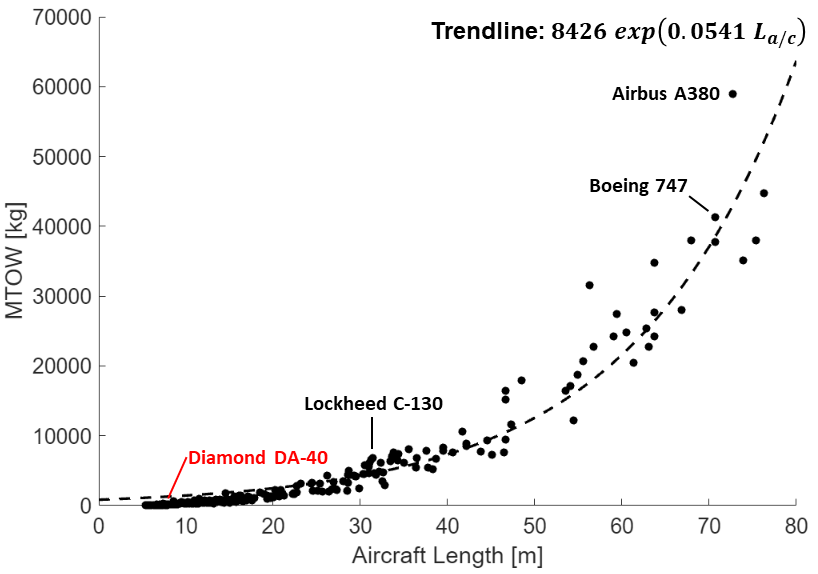
\includegraphics[width=.6\linewidth]{Figures/weights.png}
  \caption{Aircraft with a larger Max Takeoff Operating Weight (MTOW) typically have more space for more complex sensor suites compared to their General Aviation counterparts~\cite{AircraftCharacteristicsDatabase}.}
\end{figure}

Smaller aircraft are not allowed these luxuries, being manufactured with fewer sensors, overall making them less safe. Table~\ref{tbl:sensorsuitecomparison} compares the different sensors onboard a civilian airliner and a civilian general aviation aircraft.

\begin{table}[!ht]\label{tbl:sensorsuitecomparison}
  \caption{Inexhaustive list of sensors available to commercial and general aviation aircraft. (Adapted from~\cite{DiamondAircraftDA40,A380AircraftCharacteristics2020})}
  \centering
  \begin{tabular}{lcc}
    \toprule
    \textbf{Sensor}                    & \textbf{Commercial} & \textbf{General Aviation} \\
    \midrule
    Pitot Tubes                        & \(5\)               & \(2\)                     \\
    Distance Measuring Equipment       & \(2\)               & \(1\)                     \\
    Ultra-High Frequency Sensors       & \(2\)               & \(1\)                     \\
    Very-High Frequency Sensors        & \(3\)               & \(2\)                     \\
    Communication Channels             & \(2\)               & \(2\)                     \\
    Outside Air Temperature Sensors    & \(4\)               & \(1\)                     \\
    Fuel Flow Gauge                    & \(4\)               & \(1\)                     \\
    GPS receivers                      & \(2\)               & \(1\)                     \\
    Inertial Measurement Units         & \(3\)               & \(1\)                     \\
    Satellite Communications           & \(1\)               & {--}                      \\
    Specific Impulse Sensors           & \(6\)               & {--}                      \\
    Weather Radar                      & \(1\)               & {--}                      \\
    Traffic Collision Avoidance System & \(4\)               & {--}                      \\
    Radio Altimeter                    & \(3\)               & {--}                      \\

    \bottomrule
  \end{tabular}
\end{table}

Regardless of size, the sensor suite aboard any flight vehicle is able to provide measurements 50 times greater than that of a GPS receiver, so a sensor fusion algorithm is optimal for this situation. Because sensor measurements have inherit errors due to a variety of factors, they can wander or \textit{dead reckon} through time. GPS measurements, although slower, provide measurements that do not drift at cost of being slightly less accurate. Table~\ref{tbl:sensorfusionframeworks} describes the most common sensor fusion frameworks for GPS and INS platforms.
\begin{table}[!ht]\label{tbl:sensorfusionframeworks}
  \caption{Common sensor fusion frameworks used for GPS and INS collection platforms}
  \centering
  \begin{tabular}{clc}
    \toprule
    \textbf{Name}            & \textbf{Level of Measurement}          & \textbf{Typical Error} \\
    \midrule
    \textit{Loosely-Coupled} & GPS Position and Velocity              & \(1~-~3\) [m]          \\
    \textit{Tightly-Coupled} & GPS Pseudorange and Doppler            & \(1~-~2\) [m]          \\
    \textit{Deeply-Coupled}  & GPS Inphase and Quadrature Correlators & \(\leq0.5\) [m]        \\
    \bottomrule
  \end{tabular}
\end{table}
This work presents a deeply-coupled sensor fusion algorithm known as vector tracking. Of the 3 types of GPS and INS sensor fusion frameworks, it is well-documented that deeply coupled provides the most accurate localization between measurement updates~\cite{wattsGPSGLONASSL12019}.
\section{Prior Art}
The objective of this thesis is to investigate the efficacy of position estimation for a flight vehicle in GPS-degraded and GPS-denied conditions. This thesis will analyze the performance through use of a deeply-coupled sensor fusion algorithm utilizing both INS and GPS measurements. The idea of fusing INS measurements and GPS measurements together on a flight vehicle is well-documented. The following subsections scratch the surface of work performed by other authors and their contributions to the field.
\subsection{GPS and INS Sensor Fusion}

\subsection{GPS, INS, Vision Aided Sensor Fusion}

\subsection{Other Types of Flight Vehicle Sensor Fusion}

\section{Field Contributions}
The focus of the research presented in this thesis is the performance evaluation of localization in GPS-degraded and GPS denied environments for simulated low-cost sensors aboard a small general aviation fixed wing flight vehicle. Taking that into consideration, the following contributions to the field are made:
\begin{itemize}
  \item Determination of the optimal flight vehicle model to use in the navigation algorithm when considering complexity and computational performance.
  \item Comparative analysis of multiple flight scenarios reflecting realistic flight plans and GPS degradation.
  \item Analysis of deeply-coupled sensor fusion algorithm using the flight vehicle model and simulated GPS measurements to determine the efficacy of safe localization in a real-life scenario.
\end{itemize}

\section{Thesis Outline}
The rest of this work follows a description of the physical systems simulated and modeled in the FVDM, satellited simulator, and GPS receiver. After, a presentation of the results, coupled with a Monte-Carlo analysis as a performance evaluation are shown. Wrapping up, final conclusion about the investigation are made and future work considerations are presented.


\chapter{Flight Vehicle Model and Navigation Sensors}
The aircraft simulated and modelled in this thesis is the Diamond DA-40 single propeller fixed wing aircraft (Figure~\ref{fig:DA40}). Small General Aviation (GA) aircraft are easier to model compared to commercial and military aircraft as performance information for the mechanical components of the plane are not hidden through government or proprietary documents. The sections below detail the components of the Flight Vehicle Dynamic Model (FVDM) in its entirety along with the waypoint manager and navigation sensor used to modelled realistic low-cost sensor one might see aboard the actual Diamond DA-40. The simulation is a full 6 Degrees of Freedom (DOF) simulation and features 12 control inputs~-~ranging from throttle and control surface inputs to propeller pitch and mixture levers. These are covered in more detail at a later section. The chapter concludes with information about the stochastic elements in the model, which components are the aircraft they affect and the magnitude and frequency of the random walks.

\begin{figure}[!ht]\label{fig:DA40}
  \centering
  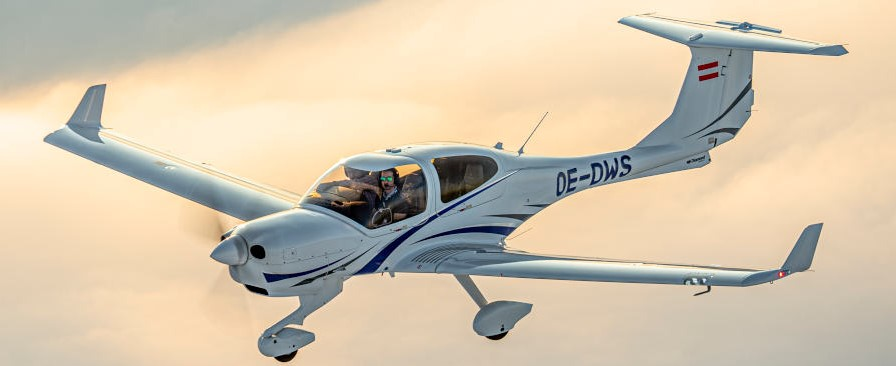
\includegraphics[width=.85\linewidth]{Figures/DA40.jpg}
  \caption{Pilot flying Diamond DA-40 single propeller aircraft~-~the focus of the collection platform for this thesis. (Adapted from~\cite{DiamondAircraftDA40}.)}
\end{figure}
\clearpage
\section{Reference Frames}
% What are reference frames
Reference frames and their transformations are a critical component to any navigation algorithm. Precise determination of a flight vehicle requires the knowledge of its position, velocity, and orientation. Reference frames describe the orientation of the flight vehicle in a global or local state. Because different components of the FVDM are physically located and oriented at unique locations of the Diamond DA-40, multiple reference frames are used to describe the forces and moments these components generate due to their placement. In order for the cumulative summation of all forces and moments generated at certain time step, reference frames transformation are used to coordinate local forces and moments into a congruent reference frame such that these calculations are performed properly. This section describes the different reference frames used in this work for the FVDM\@.
% The different reference frames on the aircraft model
% Body
\subsection{Flight Vehicle Reference Frame}
The flight vehicle reference frame or body frame describes the reference frame with origin at the center of mass of the modeled Diamond DA-40. The body frame maintains alignment shown in Figure~\ref{fig:flightvehiclereferenceframe} and remains fixed to the flight vehicle at all times. The flight vehicle reference frame is essential to the FVDM as all forces and moments are added together in the body frame before integration into global and local pose states.

\begin{figure}[!ht]\label{fig:flightvehiclereferenceframe}
  \centering
  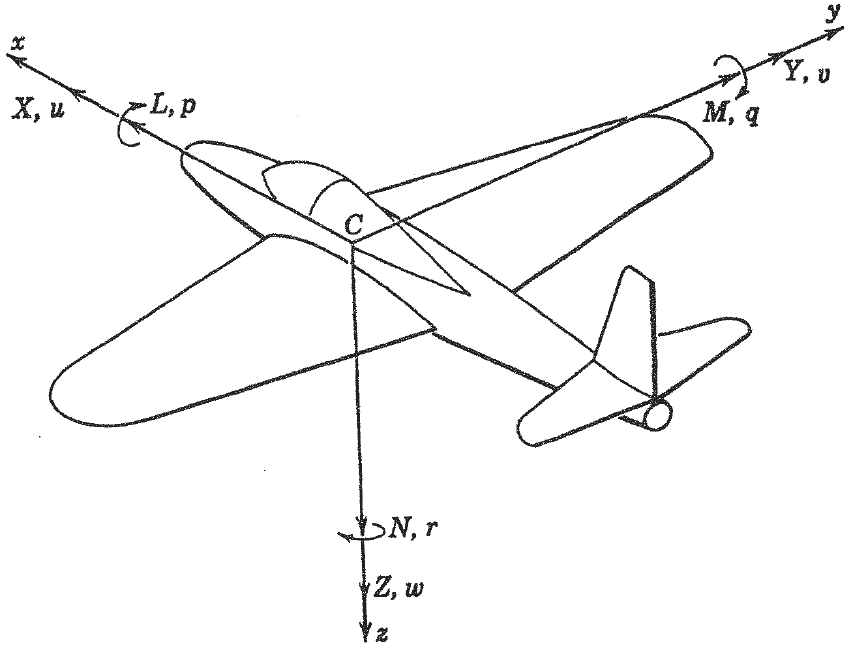
\includegraphics[width=0.85\linewidth]{Figures/bodyframe.png}
  \caption{Standard flight vehicle reference frame used in this work.~\cite{peetSpacecraftAircraftDynamics}}
\end{figure}

% Prop
\subsection{Propeller Reference Frame}
The propeller reference frame describes the axis about which the propeller rotates with origin to the propeller nacelle, as seen in Figure~\ref{fig:propnacelle}.

\begin{figure}[!ht]\label{fig:propnacelle}
  \centering
  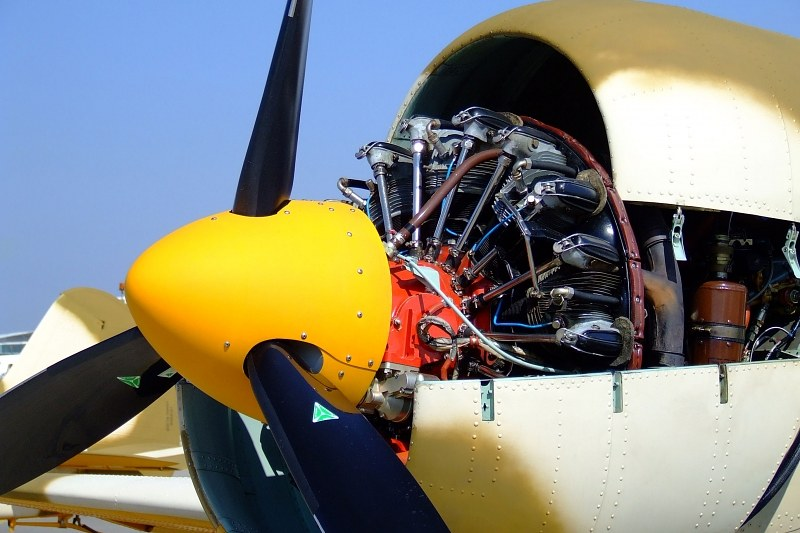
\includegraphics[width=0.65\linewidth]{Figures/propnacelle.jpg}
  \caption{Yellow propeller nacelle on the front of a general aviation aircraft.}
\end{figure}

As seen in Figure~\ref{fig:propframe}, propeller \textit{pitch}, as it is referenced in this thesis is a rotation about the \textit{y} axis, while the blades of the propeller rotate about the \textit{x} axis. This axis remains remains fixed in orientation, but always moves with the aircraft to have the same distant from the flight vehicle reference frame.\( \phi{}\) from Figure~\ref{fig:propframe} describes the twist of the blade. The blade twist is a design choice of the propeller manufacturer. The twist of the blade helps the propeller produce more thrust, but is not used in any reference frame calculations.

\begin{figure}[!ht]\label{fig:propframe}
  \centering
  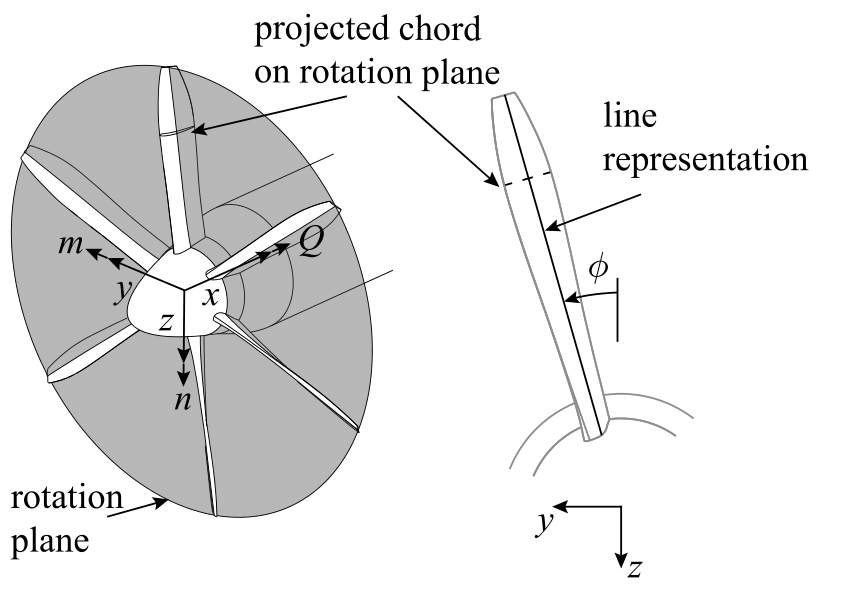
\includegraphics[width=0.75\linewidth]{Figures/propframe.png}
  \caption{The reference frame used to model the dynamic of the propeller in this work~\cite{vanarnhemEngineeringMethodEstimate2020}.}
\end{figure}

% Wind
\subsection{Local Wind Axes Reference Frame}
The local wind axes reference frame is used to calculate the lift and drag generated from their respective components with origin at the center of mass of the modeled Diamond DA-40. The orientation of the reference frame changes such that \(\Psi \) remains parallel with the trajectory of the aircraft and \(\alpha \) remains parallel to the ground below. In literature, \( \Psi \) and \(\alpha \) are referred to as the \textit{sideslip} and \textit{angle of attack} of the aircraft during flight.

\begin{figure}[!ht]\label{fig:windframe}
  \centering
  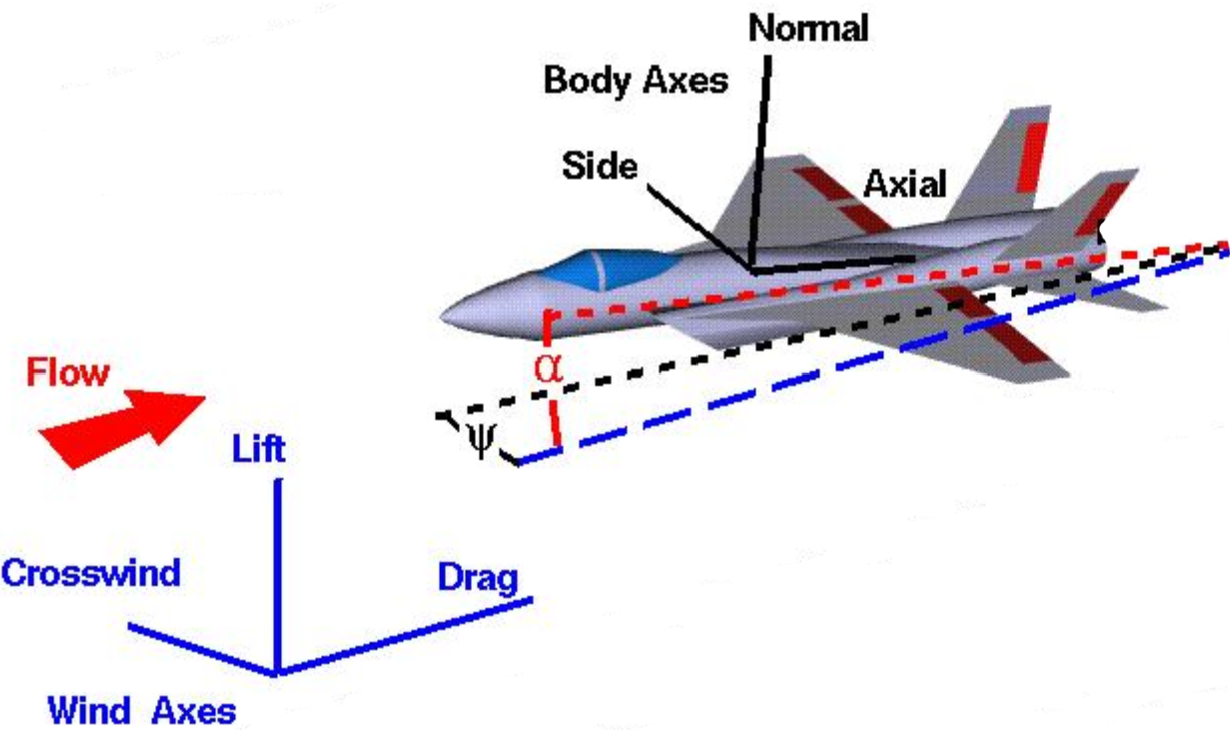
\includegraphics[width=0.75\linewidth]{Figures/windaxes.png}
  \caption{Flight vehicle reference frame and local wind reference frame (dotted lines) (Adapted from~\cite{ForceBalanceCoordinates}).}
\end{figure}

% Local
\subsection{Local Navigation Reference Frame}
A local navigation frame is necessary to define the orientation of the flight vehicle. This work implements a North-East-Down reference frame in which the axes are aligned with the topographic directions: North, East, and vertical as seen in Figure~\ref{fig:NEDframe}. The origin of the local reference frame is defined at the initial position in the flight vehicle dynamics model and the navigation algorithm. The Euler attitude angles are used to describe the orientation of the Diamond DA-40 relative to the local navigation frame. When the aircraft has no roll pitch, or yaw, this equates to the aircraft flying perfectly tangential to Earth's ellipsoid, with the nose of the aircraft pointing towards the North.

\begin{figure}[!ht]\label{fig:NEDframe}
  \centering
  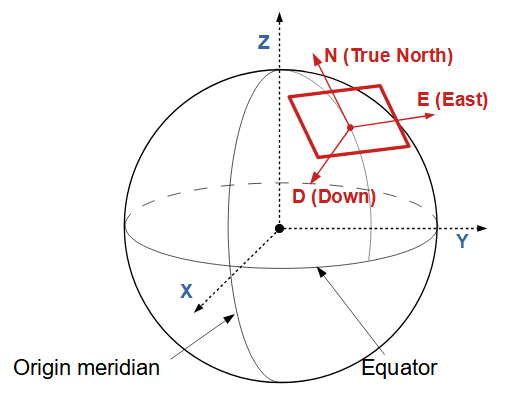
\includegraphics[width=0.75\linewidth]{Figures/nedframe.PNG}
  \caption{North-East-Down Reference Frame~-~the local reference frame used in this thesis.}
\end{figure}

\subsection{Global Reference Frames}
Global Reference Frames are critical for GPS receiver to calculate position and velocity. In summary, a position from a receiver is based on distances between the receiver and any visible satellites. As all GPS satellites operate in orbit around the Earth, the global reference frame provides a suitable solution that encompasses both satellite and receiver position and velocities. In this thesis, two global reference frames are used. The Earth-Centered, Earth-Fixed (ECEF) and the geodetic reference system (referred to as LLA from now on). The ECEF reference frame is considered the standard global reference frame used as it works well for defining both positions and velocities for satellites and receivers, but falls short when it comes to visualization as the origin of the ECEF frame is the center of the Earth. An alternative reference frame, LLA, allows a visualization advantage by defining positions based on the surface of the Earth. Both LLA and ECEF reference frames utilize the World Geodetic System 1984 (WGS84) to describe Earth's geoid and gravitational field as function of parameters in Table~\ref{tbl:wgs84}. Visualization of both reference frames can be seen in Figure~\ref{fig:globalframes}.

\begin{table}[!ht]\label{tbl:wgs84}
  \caption{Properties describing the WGS84 ellipsoid}
  \centering
  \begin{tabular}{cccc}
    \toprule
    \textbf{Property}          & \textbf{WGS84 Value} & \textbf{Units} \\
    \midrule
    Equatorial Radius, \(R_0\) & 6,378,137.0          & meters         \\
    Polar Radius, \(R_P\)      & 6,356,752.31425      & meters         \\
    Flattening, \(f\)          & 1/298.257223563      &                \\
    Eccentricity, \(e\)        & 0.0818181808425      &                \\
    \bottomrule
  \end{tabular}
\end{table}

\begin{figure}[!ht]\label{fig:globalframes}
  \centering
  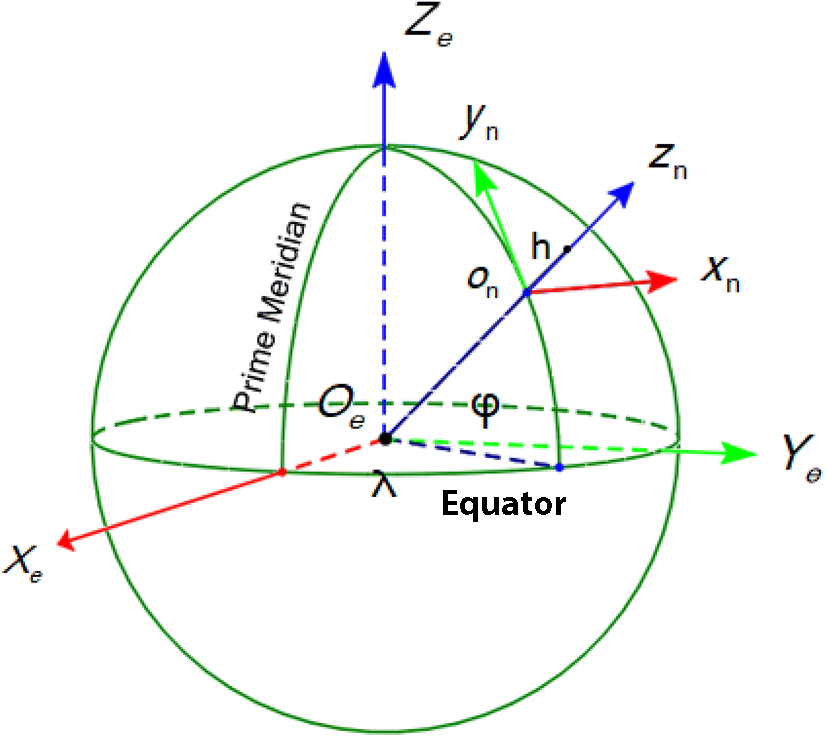
\includegraphics[width=0.75\linewidth]{Figures/globalframe.png}
  \caption{ECEF and geodetic reference frames as used in this thesis.}
\end{figure}

% How the reference frames are calculated (DCMs)
\clearpage
\section{Reference Frame Transformations}
Reference frame transformations are critical to any sensor fusion algorithm in order to properly add vectors of different frames together. Reference frame transformations range in complexity, the simplest being a transformation of the NED frame into the East-North-Up reference frame. A more complex transformation could be the global ECEF frame into the body frame and vice versa. The reference frame transformation used in this thesis are described in the following subsections.

\subsection{ECEF to LLA}

One of the more complicated reference frame transformations is between the two global frames, ECEF and LLA\@. The conversion from LLA to ECEF is provided first in Equations~\ref{eq:meridiancurvature},~\ref{eq:transversecurvature},~\ref{eq:lla2ecefx},~\ref{eq:lla2ecefy}, and~\ref{eq:lla2ecefz}. The variables within these equations are defined in Table~\ref{tbl:wgs84}.

\begin{equation}\label{eq:meridiancurvature}
  R_N (L) = \frac{R_0 \, \left(1 - e^2\right)}{{\left(1 - e^2 \, \sin^2 {\left(L\right)}\right)}^{3/2}}
\end{equation}

Equation~\ref{eq:meridiancurvature}, \(R_N (L)\) describes the one the two radii of curvature. In this case, the meridian radius of curvature describes the north to south motion. The second radii of curvature (Equation~\ref{eq:transversecurvature}) describes the east to west motion and is known as the transverse radius of curvature (\(R_E (L) \)).

\begin{equation}\label{eq:transversecurvature}
  R_E (L) = \frac{R_0}{\sqrt{1 - e^2 \, \sin^2 {\left(L\right)}}}
\end{equation}

After the transverse radius of curvature is calculated, it used with the LLA positions to calculate the ECEF \(X\), \(Y\), and \(Z\) positions as shown in Equations~\ref{eq:lla2ecefx},~\ref{eq:lla2ecefy}, and~\ref{eq:lla2ecefz}.

\begin{equation}\label{eq:lla2ecefx}
  X_{ECEF} = \left(R_E (L) + h\right) \, \cos \left(L\right) \, \cos \left(\lambda\right)
\end{equation}

\begin{equation}\label{eq:lla2ecefy}
  Y_{ECEF} = \left(R_E (L) + h\right) \, \cos \left(L\right) \, \sin \left(\lambda\right)
\end{equation}

\begin{equation}\label{eq:lla2ecefz}
  Z_{ECEF} = \left[\left(1 - e^2\right) \, R_E (L) + h\right] \sin \left(L\right)
\end{equation}

The ECEF to LLA conversion is more complicated. In order to calculate \(L\) in Equation~\ref{eq:ecef2llaL}, \(h\) from Equation~\ref{eq:ecef2llaaltitude} must be calculated {--} and vice versa. The correct way to solve for positions in the LLA reference frame is iteratively until the difference between positions from iteration to iteration is near-zero.

\begin{equation}\label{eq:ecef2llaL}
  L = \textrm{atan2}\left(\frac{Z_{ECEF} \left[R_E (L) + h\right]}{\sqrt{X_{ECEF}^2 + Y^2_{ECEF}} \, \left[ \left(1 - e^2\right) R_E (L) + h\right]}\right)
\end{equation}

\begin{equation}\label{eq:ecef2llalambda}
  \lambda = \textrm{atan}\left(\frac{Y_{ECEF}}{X_{ECEF}}\right)
\end{equation}

\begin{equation}\label{eq:ecef2llaaltitude}
  h = \frac{\sqrt{X_{ECEF}^2 + Y^2_{ECEF}}}{\cos\left(L\right)} - R_E (L)
\end{equation}


\subsection{ECEF to Local}
The conversion from the ECEF reference frame to the local navigation reference frame can be done by forming a Direction Cosine Matrix (DCM),

\begin{equation}\label{eq:ECEF2LNDCM}
  C^{\textrm{LN}}_{\textrm{ECEF}} =
  \begin{bmatrix}
    -\sin\left(L\right)\cos\left(\lambda\right) & -\sin\left(L\right)\sin\left(\lambda\right) & \cos\left(L\right)  \\
    -\sin\left(\lambda\right)                   & \cos\left(\lambda\right)                    & 0                   \\
    -\cos\left(L\right)\cos\left(\lambda\right) & -\cos\left(L\right)\sin\left(\lambda\right) & -\sin\left(L\right) \\
  \end{bmatrix},
\end{equation}

and then multiplying the ECEF position vector to produce a position in the NED frame as discussed previously. In Equation~\ref{eq:ECEF2LNDCM}, \(C^{\textrm{LN}}_{\textrm{ECEF}}\) describes the DCM used for the transformation. The notation follows such that the subscript (ECEF) is the position in the original reference frame and the superscript (LN) is the reference frame the position is being rotated into. This thesis will always follow this notation to avoid any confusion.

\subsection{Local to Body}
Similar to the conversion of ECEF to the local navigation frame, the conversion from the local navigation to the flight vehicle reference frame can be done by forming the DCM (Equation~\ref{eq:321DCM}).
\begin{equation}\label{eq:321DCM}
  C^{\textrm{FV}}_{\textrm{LN}} =
  \begin{bmatrix}
    \textrm{c}_{\theta}\textrm{c}_{\psi}                                                        & \textrm{c}_{\theta}\textrm{s}_{\psi}                                                        & -\textrm{s}_{\theta}                 \\
    -\textrm{c}_{\phi}\textrm{s}_{\psi} + \textrm{s}_{\phi}\textrm{s}_{\theta}\textrm{c}_{\psi} & \textrm{c}_{\phi}\textrm{c}_{\psi} + \textrm{s}_{\phi}\textrm{s}_{\theta}\textrm{s}_{\psi}  & \textrm{s}_{\phi}\textrm{c}_{\theta} \\
    \textrm{s}_{\phi}\textrm{s}_{\psi} + \textrm{c}_{\phi}\textrm{s}_{\theta}\textrm{c}_{\psi}  & -\textrm{s}_{\phi}\textrm{c}_{\psi} + \textrm{c}_{\phi}\textrm{s}_{\theta}\textrm{s}_{\psi} & \textrm{c}_{\phi}\textrm{c}_{\theta} \\
  \end{bmatrix}
\end{equation}
In this case, the DCM comprises of the 3 Euler angles {--} roll (\( \phi \)), pitch (\( \theta \)), and yaw (\( \psi \)). To allow the matrix to fit the width of the paper, \textit{c} and \textit{s} denote the \textit{cosine} and \textit{sine} trigonometric functions, respectively.

If one wanted to convert position from the flight vehicle to ECEF reference frame, multiplying Equations~\ref{eq:321DCM} and~\ref{eq:ECEF2LNDCM} provides the user with a DCM to do this (Equation~\ref{eq:ECEF2BODY}).

\begin{equation}\label{eq:ECEF2BODY}
  C^{\textrm{FV}}_{\textrm{ECEF}} = C^{\textrm{FV}}_{\textrm{LN}} \, C^{\textrm{LN}}_{\textrm{ECEF}}
\end{equation}

It should be noted that any of these DCM reference frame transformations can be inverted by simply transposing the matrices.

\clearpage
\section{Dynamic Vehicle Model}
This section describes the implementation of each key component in generating the forces and moments that propel the flight vehicle model forward during flight. There are 4 main components need to simulate the aircraft at high-fidelity. The engine and propeller models serve as the main proponents in accelerating the air around the aircraft, further allowing the aerodynamic model to provide lift. The performance of both the aerodynamics and engine models are based on the condition of the ambient atmosphere that are described by the ISA atmosphere model. The section holds several subsections that describe these systems and the equations that govern them.

\subsection{Atmosphere Model}\label{section:atmos}
In order to more accurately calculate a handful of dynamics models studied in this work, a model of Earth's atmosphere is needed to provided ambient temperature, pressure, density, speed of sound, and wind. This thesis uses the International Standard Atmosphere (ISA) model to approximate ambient temperature, ambient pressure, ambient density, and the speed of sound given a certain height above Mean Sea Level (MSL). Using an assumed linear distribution for temperature as a function of altitude, the ISA model assumes hydrostatic equilibrium as seen by Equation~\ref{eq:2.1},

\begin{equation}
  \frac{dP}{dh} = -\rho \, g,
  \label{eq:2.1}
\end{equation}

where \(\frac{dP}{dh}\) is the vertical pressure gradient as a factor of air density, \( \rho \), and Earth's gravity, \(g\). After integrating Equation~\ref{eq:2.1}, the ISA model uses the ideal gas law (Equation~\ref{eq:2.2})

\begin{equation}
  P = \rho \, R\textsubscript{air} \, T
  \label{eq:2.2}
\end{equation}

to solve for the ambient pressure \(P\), and density, \( \rho \). A complete form of the ISA model is seen in Equations~\ref{eq:2.3} and~\ref{eq:2.4}.

\begin{equation}
  P = P_0\,\exp\left({\frac{-g\,\Delta h}{R\textsubscript{air}\,T}}\right)
  \label{eq:2.3}
\end{equation}

\begin{equation}
  \rho = \rho_0\,\exp\left({\frac{-g\,\Delta h}{R\textsubscript{air}\,T}}\right)
  \label{eq:2.4}
\end{equation}

where \(P_0\) and \(\rho_0\) are atmospheric layer values for pressure and density, respectively; \(R\textsubscript{air}\) is the specific gas constant for air and \(\Delta h\) is difference between the current altitude of the flight vehicle and altitude of the current atmospheric layer. The speed of sound is a function of temperature and can be calculated using Equation~\ref{eq:2.5}

\begin{equation}
  a = \sqrt{\gamma \, R\textsubscript{air}\,T},
  \label{eq:2.5}
\end{equation}

where \(a\) is the speed of sound in meters per second and \( \gamma \) is the ratio of specific heats. Figure~\ref{fig:atmos} describes these atmospheric parameters from MSL to 85,000 meters above sea level.

Along with the aforementioned atmospheric parameters, wind is a vital modeling parameter for flight vehicles. For smaller SWAP flight vehicles, small gusts of wind can greatly affect their dynamics~\cite{raymerAircraftDesignConceptual2018}. This thesis uses an updated version of the Horizontal Wind Model~\cite{drobEmpiricalModelEarth2008,drobUpdateHorizontalWind2015} using collected satellite data from the Nation Oceanic and Atmospheric Administration (NOAA). The model accepts the current position of the flight vehicle to provide a predicted wind vector in the meridional and zonal reference frame. Implementation of the ISA model and calculation of winds can be found under \textit{Atmosphere.m} in~\cite{millerNsm0014thesis1969}.

\subsection{Piston Engine Model}
% Overview of Piston and Propeller Model
Small general aviation aircraft generate propulsive forces through use of an engine that spins a shaft which is connected to a propeller. The engine modeled and simulated is a piston, air-cooled engine. The typical aircraft piston engine is modeled as a four-stroke otto cycle~\cite{raymerAircraftDesignConceptual2018}. The otto cycle is a well-known thermodynamic theory that relies on a large air mass flow rate to generate power~\cite{gudmundssonGeneralAviationAircraft2014}. The components of the engine that produce the power are described below.

% Manifold Pressure
Because the engine is air-cooled, one of more important component is the engine manifold. The engine inlet manifold is a set of vents that allow the ambient air to feed directly into the combustion chambers where the oxygen in the air is used in combination with the fuel to generate power. Based on the commanded throttle input, these manifold vents can be closed or open to let in more or less air, and in return the engine delivers a proportional amount of power to the shaft. The power production from the engine is heavily reliant on the density of air. The Gagg and Ferrar model,

\begin{equation}\label{eq:gaggandferrar}
  \textrm{power} = \textrm{power}_{0}\left(\frac{\rho}{\rho_0} - \frac{1 - \rho/\rho_0}{7.55}\right),
\end{equation}

relates power production to the density of air. Where \(rho\) is the density of the ambient air as a function of altitude (Section~\ref{section:atmos}), \(rho_0\) is the density of ambient air at sea-level on a standard day, and \(\textrm{power}\) is the max engine power provided the density ratio and the nominal power production of the engine. From~\cite{1590000APdf}, the engine modeled in this work has a nominal power output on a sea-level standard day of 600 horsepower (447.42 kiloWatts). Figure~\ref{fig:gaggferrar} shows the power output of the engine modeled in this thesis based on the Gagg and Ferrar model and nominal sea-level power production.

\begin{figure}[!ht]\label{fig:gaggferrar}
  \centering
  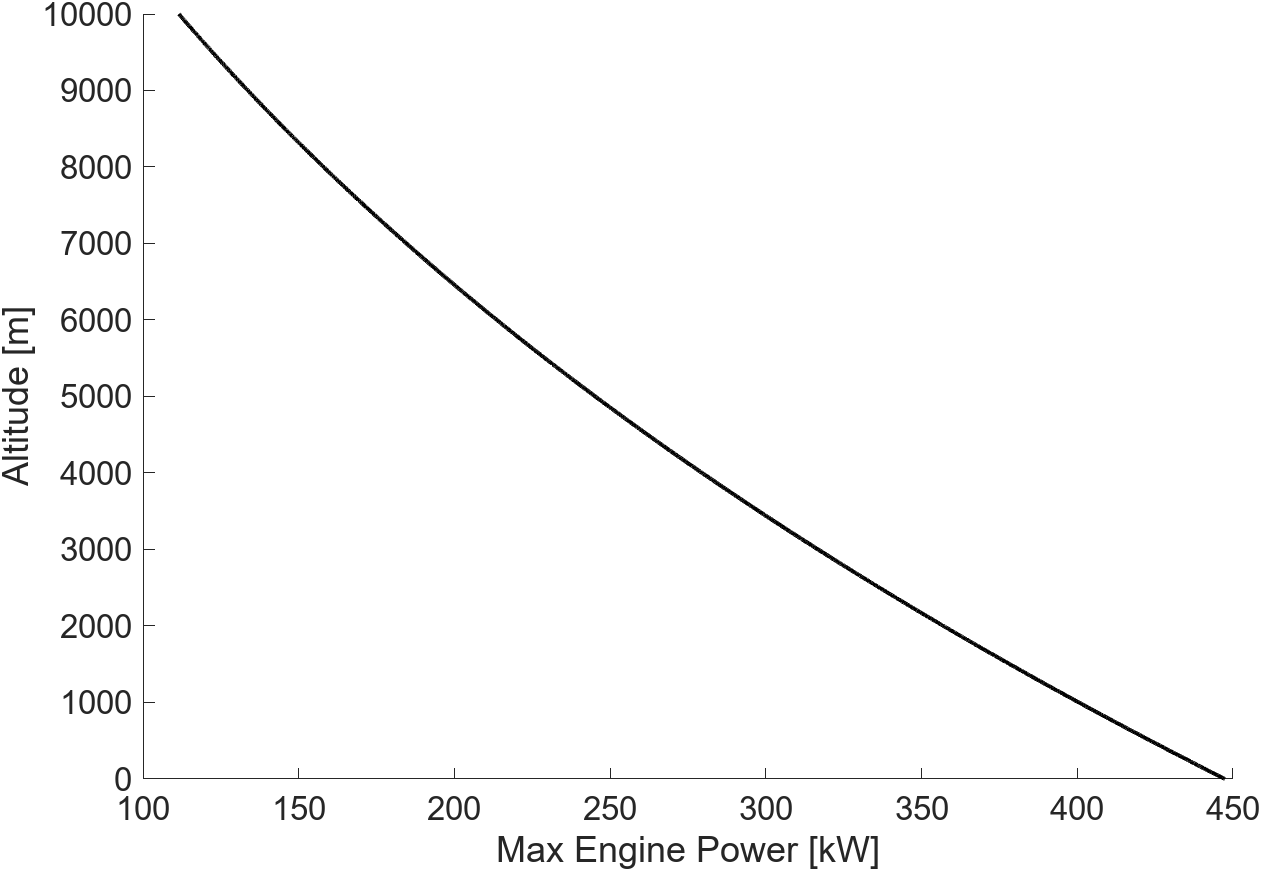
\includegraphics[width=0.85\linewidth]{Figures/gaggferrar.png}
  \caption{Power output for modeled engine as a function of aircraft altitude.}
\end{figure}

However, not all power generated by the engine is absorbed by the shaft. There are losses that include shaft slippage or uneven distribution of fuel in the combustion chamber. These \"errors\" are modeled as a \textit{Power Factor} and compares the the ideal power produced by the engine to the power absorbed by the shaft. This proportional amount is queried at every time step in the simulation as seen in Figure~\ref{fig:PFLUT}.

\begin{figure}[!ht]\label{fig:PFLUT}
  \centering
  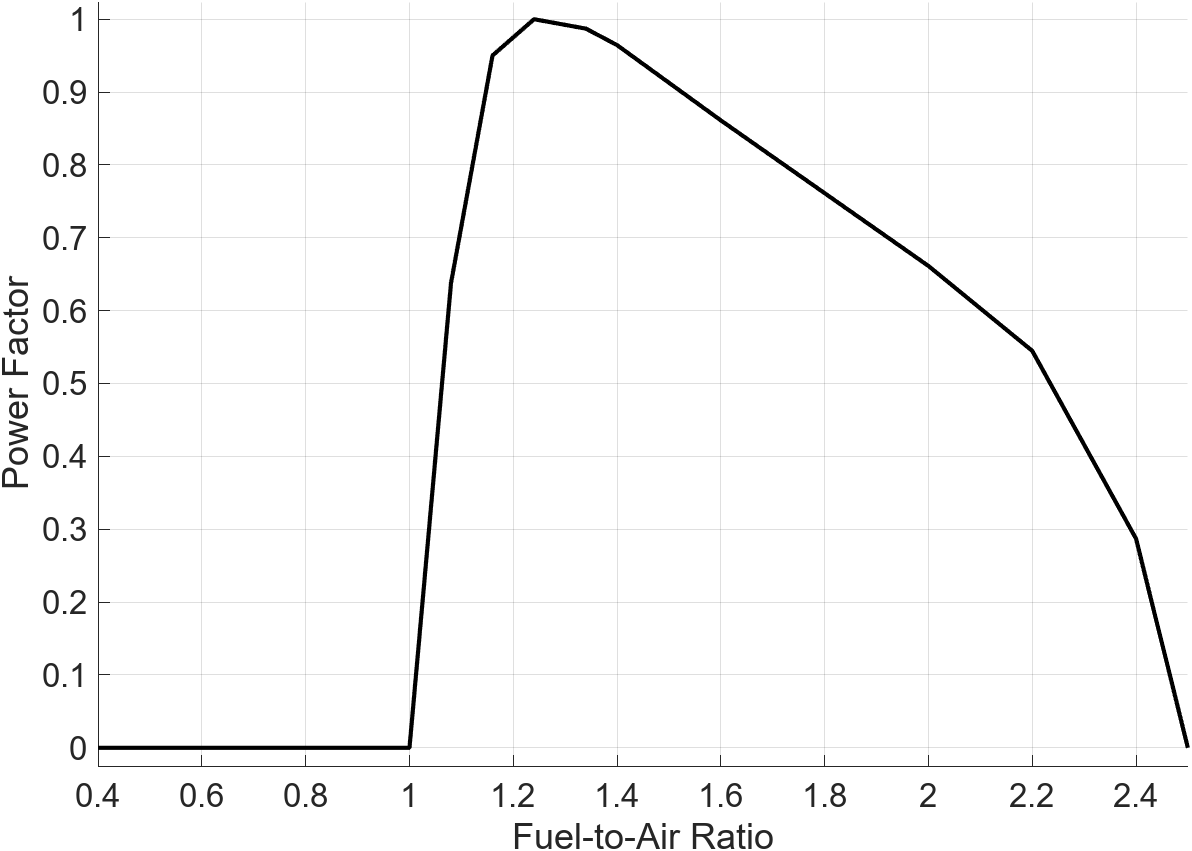
\includegraphics[width=.75\linewidth]{Figures/PFLUT.png}
  \caption{Power factor look up table for modeled engine.}
\end{figure}

% Electric Governor Model
The governor that exists in ground and flight vehicles exists such that drastic changes in throttle do not result in extreme ramps of torque that could structurally damage engine components. It limits the rate of commanded throttle to be linear so that rotational acceleration of the shaft and propeller is safely increased or decreased. The governor also controls fuel consumption of the engine by controlling the engine speed. The fuel consumption is queried at every time step using a look up table that is calculated before the simulation starts (Figure~\ref{fig:BSFCLUT}).

\begin{figure}[!ht]\label{fig:BSFCLUT}
  \centering
  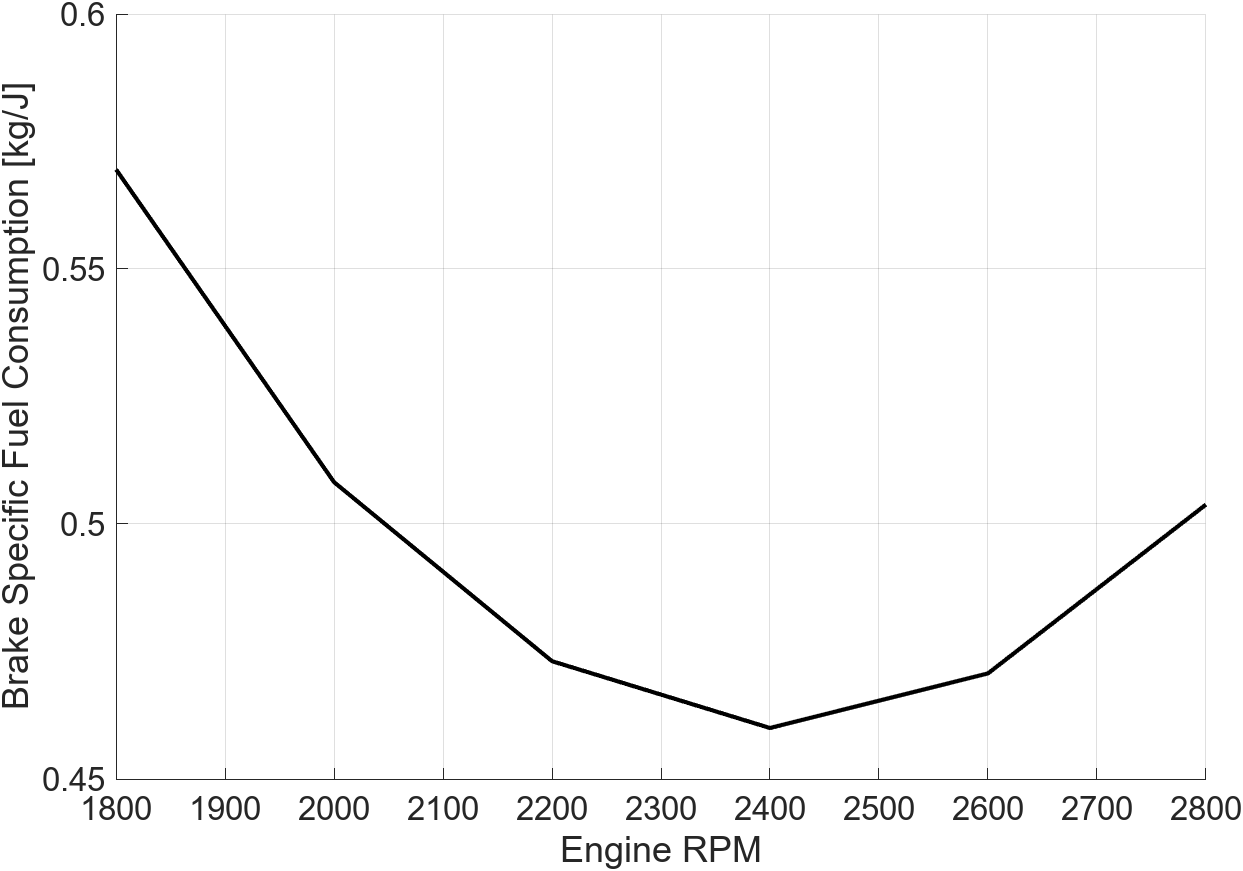
\includegraphics[width=.75\linewidth]{Figures/BSFCLUT.png}
  \caption{Brake specific fuel consumption look up table for modeled engine.}
\end{figure}

\subsection{Propeller Modeling}
% Propeller Dynamics
The purpose of an aircraft propeller is to increase the velocity of the ambient air around them such that the lifting surfaces on the aircraft can generate lift and keep the aircraft in flight. There are 3 main components to focus on when designing and manufacturing propellers. These are
\begin{itemize}
  \item[i.] Materials
  \item[ii.] Number of Blades
  \item[iii.] Blade Geometry.
\end{itemize}
While the focus of this thesis is not on details in propeller design, it is important to show how the history and differences between each of these 3 items affect the efficiency and performance a propeller has in generating thrust power for the aircraft. The first modern propeller were designed in the early 1900's. Originally made of wood, they featured 3 blades and crudely resembled airfoil shapes (Figure~\ref{fig:woodprops}).

\begin{figure}[!ht]\label{fig:woodprops}
  \centering
  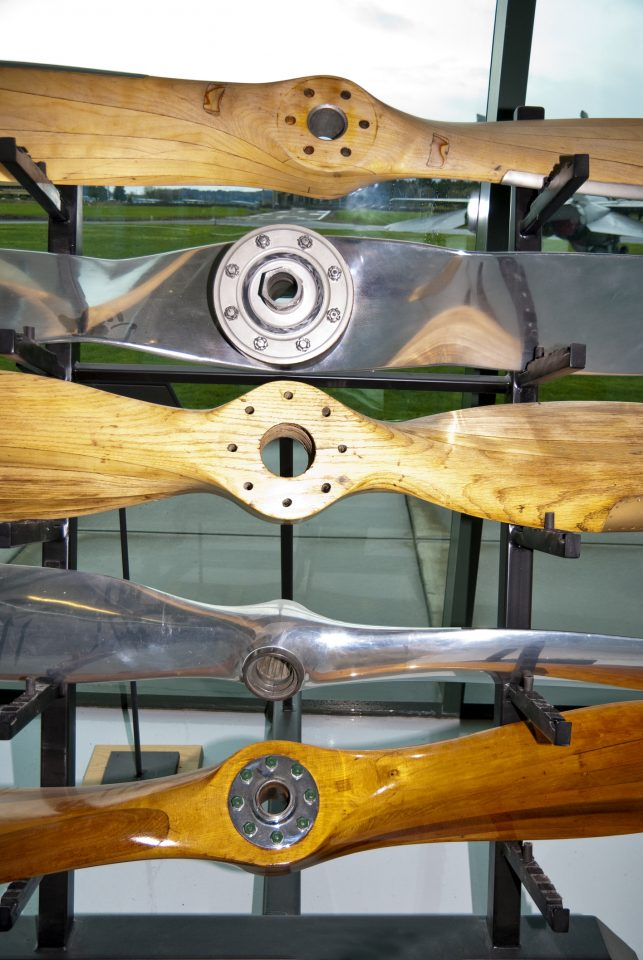
\includegraphics[width=0.3\linewidth]{Figures/woodProps.jpg}
  \caption{Collection of historic wood and steel propellers~\cite{ianHowIdentifyHistoric2016}.}
\end{figure}

These propellers had a fixed pitch, meaning they could not rotate up and down during flight~-~severely costing the propeller thrust power. In 1929, Wallace Turnbull invented the variable pitch propeller, allowing pilots to control the pitch the propeller, dramatically increasing propeller efficiency during flight~\cite{ianShortHistoryAircraft2018}. Through time and the advent of computers, Computational Fluid Dynamics (CFD) analyses shaped a handful of equations that define the performance and efficiency of a propeller design. In this work, a 3-blade Hartzell~\cite{HartzellPropellerInc} composite propeller is used as it is the Original Equipment Manufacturer (OEM) propeller on the Diamond DA-40 aircraft. This propeller is a variable-pitch constant speed propeller, meaning the pitch of the propeller is optimally adjusted for the current flight condition, while at the same time, maintaining a constant rotational speed to conserve fuel and hold a consistent propeller efficiency (Equation~\ref{eq:propellerefficiency}).

Before the simulation is started, the propeller is analyzed through \textit{FlightStream}~\cite{FlightStream}, a surface vorticity flow solver, to analyze the propeller for its lift coefficient (\(C_L\)) at varying flight conditions (Figure~\ref{fig:flightstreamprop}).

\begin{figure}[!ht]\label{fig:flightstreamprop}
  \centering
  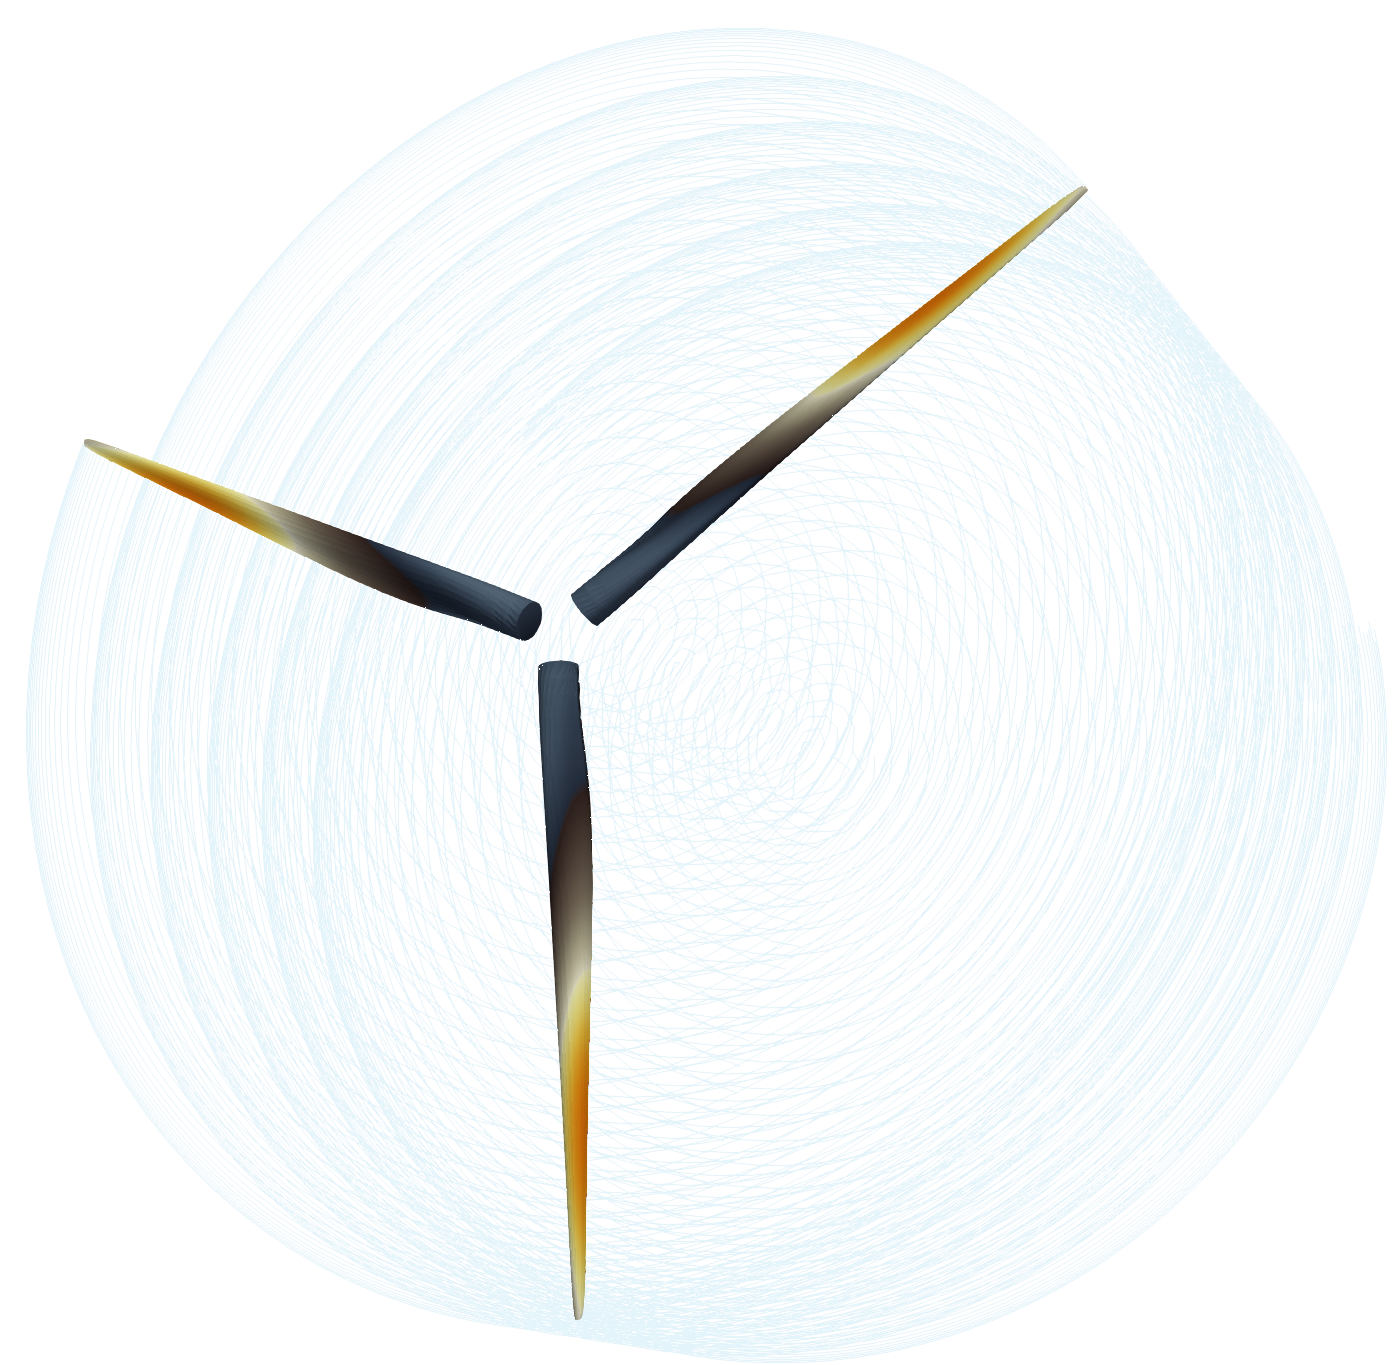
\includegraphics[width=.35\linewidth]{Figures/flightstreamprop.png}
  \caption{Analyzing 3-blade propeller through Flightstream~\cite{FlightStream}.}
\end{figure}

Once the lift coefficient is determined, numerical look up tables are generated such that the calculation of the forces and moments generated by the propeller can be interpolated, allowing the simulation to be run in real time. To determine the amount of thrust and torque generated by the propeller, the \textit{Activity Factor} (Equation~\ref{eq:activityfactor}) of the propeller must first be determined. The \textit{Activity Factor} is a measures of the propellers ability to absorb propeller and the effectiveness of each blade's width.

% Activity Factor
\begin{equation}\label{eq:activityfactor}
  AF_{\textrm{per blade}} = \frac{1 \times 10^5 \, c_{\textrm{root}}}{16 \, D} \left(0.25 + 0.2 \, \lambda - 0.2 \right)
\end{equation}

Where \(AF_{\textrm{per blade}}\) is the \textit{Activity Factor} per blade, \(c_{\textrm{root}}\) is the length of a blade's chord at the root, \(D\) is the diameter of the propeller, and \( \lambda \) is the taper ratio, described in Section~\ref{section:aerodynamic}. Table~\ref{tbl:propparams} describes the design characteristics of the propeller used in this thesis.

\begin{table}[!ht]\label{tbl:propparams}
  \caption{Characteristics of the propeller modeled for this work.}
  \centering
  \begin{tabular}{cccc}
    \toprule
    Characteristics       & Value  & Units  \\
    \midrule
    \(c_{\textrm{root}}\) & 0.1475 & meters \\
    \(D\)                 & 1.9    & meters \\
    \( \lambda \)         & 0.8    & N/A    \\
    \(C_L\)               & 0.5    & N/A    \\
    \bottomrule
  \end{tabular}
\end{table}

Because the dimensions of the propeller are known, we can determine the \textit{Activity Factor} of the blade to be (Equation~\ref{eq:activityfactorcalc},~\ref{eq:activityfactorcalc2})

% Activity Factor Calculation
\begin{equation}\label{eq:activityfactorcalc}
  AF_{\textrm{per blade}} = \frac{1 \times 10^5 \, (0.1475)}{16 \, (1.9)} \left(0.25 + 0.2 \, (0.8) - 0.2 \right)
\end{equation}

\begin{equation}\label{eq:activityfactorcalc2}
  AF_{\textrm{per blade}} = 101.89.
\end{equation}

Now that the \textit{Activity Factor} is known for the modeled propeller. The \textit{Power} (Equation~\ref{eq:powercoefficient}) and \textit{Thrust} (Equation~\ref{eq:thrustcoefficient}) coefficients can be calculated to show how well the propeller generates thrust when the aircraft is static (\i.e.\ starting takeoff). For this analysis, we assume the engine to be producing a nominal \(600\) horsepower (\(447.42\) [kW]) and applying a torque equivalent to \(2200\) [rpm] (\(36.6\) [rev\(/\)s]).

% Power Coefficient
\begin{equation}\label{eq:powercoefficient}
  c_P = \frac{P}{\rho \, n^3 \, D^5}
\end{equation}

% Thrust Coefficient
\begin{equation}\label{eq:thrustcoefficient}
  c_T = \frac{T}{\rho \, n^2 \, D^4}
\end{equation}

In Equations~\ref{eq:powercoefficient} and~\ref{eq:thrustcoefficient}, \(P\) is the engine power, denoted in kiloWatts, \(n\) is the rotational speed of the shaft, denoted in revolutions per second, \(T\) is the thrust of the propeller, denoted in kiloNewtons, and \( rho \) is density of the ambient air. For these calculations, an assume sea-level density is used (1.225 [\(kg/m^3\)]). Using Figure~\ref{fig:staticpropthrust} and our nominal engine power and torque output, we can approximate the thrust coefficient (Equations~\ref{eq:calcCT1},~\ref{eq:calcCT2},~\ref{eq:calcCT3} and~\ref{eq:calcCT4}).

\begin{figure}[!ht]\label{fig:staticpropthrust}
  \centering
  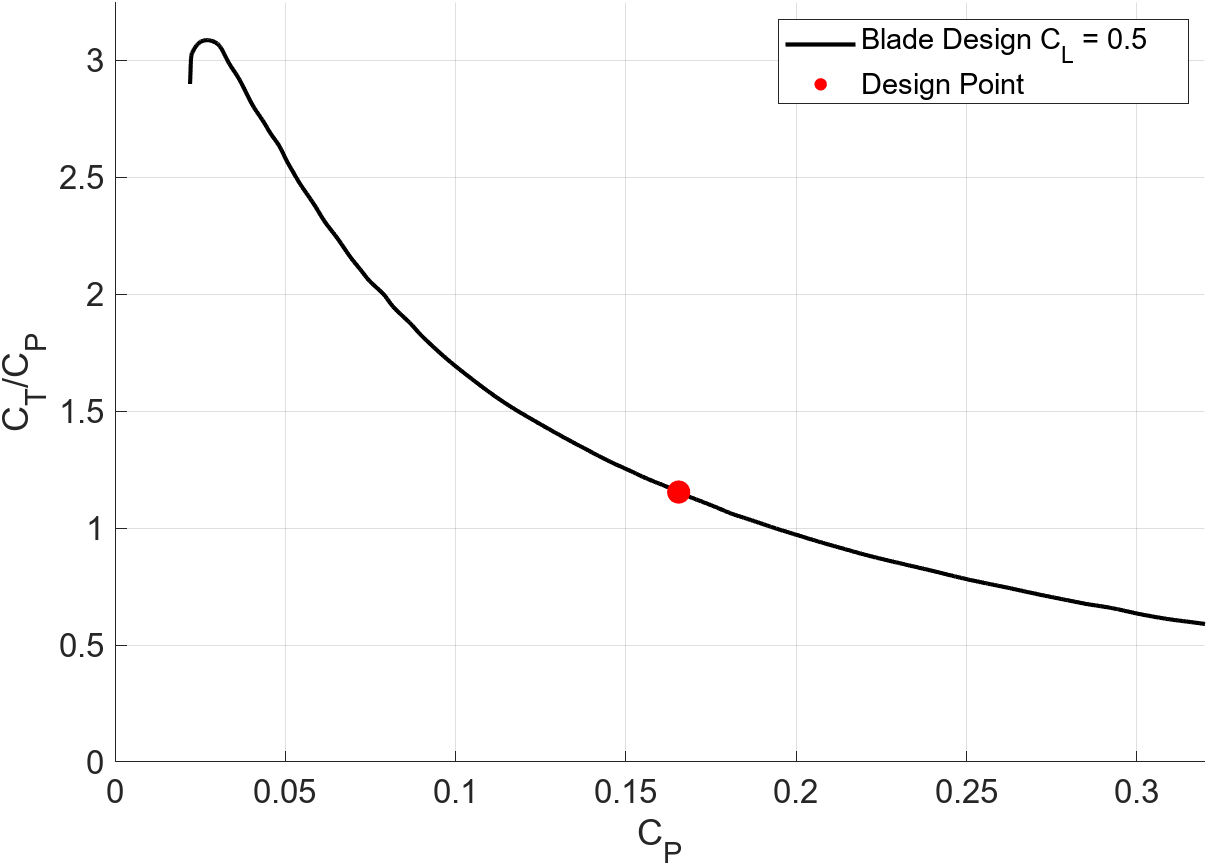
\includegraphics[width=0.85\linewidth]{Figures/StaticThrust.png}
  \caption{Static propeller thrust for the modelled propeller (Adapted from~\cite{GeneralizedMethodPropeller}).}
\end{figure}

\begin{equation}\label{eq:calcCT1}
  c_P = \frac{(447.42)(550)}{{(1.225)} \, {(36.6)}^3 \, {(1.9)}^5}
\end{equation}
\begin{equation}\label{eq:calcCT2}
  c_P = 0.16547
\end{equation}
\begin{equation}\label{eq:calcCT3}
  \frac{C_T}{C_P}(@C_P == 0.16547) = 1.1544
\end{equation}
\begin{equation}\label{eq:calcCT4}
  C_T = 0.18997
\end{equation}


Mapping \(C_T\) and \(C_P\) allows for computationally inexpensive queries with calculating propeller efficiency during flight (Equation~\ref{eq:propellerefficiency}).
% Propeller Efficiency
\begin{equation}\label{eq:propellerefficiency}
  \eta_P = \frac{C_T}{C_P} \, J
\end{equation}

Propeller efficiency, \( \eta_P \) compares the amount of power produced by the engine and shaft to the amount of power applied to the ambient air~-~an ideal propeller efficiency would be \(1\), where all of the produced engine power is used to accelerate the ambient air. The \textit{Advance Ratio}, \(J\)
% Advance Ratio
\begin{equation}\label{eq:advanceRatio}
  J = \frac{V}{n \, D} \, ,
\end{equation}

describes how far the flight vehicle moves at each full revolution of the propeller.
\(V\) is the forward velocity of the flight vehicle, \(n\) is the rotational speed of the propeller and \(D\) is the propeller diameter.

The final step in calculating the forces and moments generated by the propeller is querying the thrust based on the previous equations (Equation~\ref{eq:thrust}).
% Thrust
\begin{equation}\label{eq:thrust}
  T = \frac{P \, \eta_P}{V}
\end{equation}

A handful of steps, provided below, list the necessary calculations needed to simulate the thrust for the Diamond DA-40 modeled in this thesis. Because of some of the quantities are constant (i.e.\ propeller diameter and lift coefficient), look up tables can be created before hand to lower the computational load.

\begin{itemize}
  \item[1.] Calculate Activity Factor for given propeller design (Equation~\ref{eq:activityfactor}).
  \item[2.] Query coefficients data table (Figure~\ref{fig:staticpropthrust}) to define \textit{Power} and \textit{Thrust} coefficients (Equations~\ref{eq:powercoefficient} and~\ref{eq:thrustcoefficient}).
  \item[3.] Query \textit{Advance Ratio} (Equation~\ref{eq:advanceRatio}) data table for given flight velocity and shaft rotational speed.
  \item[4.] Calculate \( \eta_P \) (Equation~\ref{eq:propellerefficiency}), for given \(J\), \(C_P\), and \(C_T\).
  \item[5.] Calculate \(T\) using Equation~\ref{eq:thrust}.
  \item[6.] The moment generated by the propeller is simply the cross-product between the thrust and moment arm between the tip of the propeller and the nacelle of propeller.
\end{itemize}

\subsection{Aerodynamic Modeling}\label{section:aerodynamic}
% Section Overview
In all phases of flight, aircraft must be efficient at generating lift forces on the airframe to sustain flight. Since the early 1920's, the National Advisory Committee for Aeronautics (NACA) started tested oblique elliptical shapes in wind tunnels known as \textit{airfoils}. Airfoils affect all aspects of flight including cruise speed, takeoff and landing speed and distance, and overall aerodynamic efficiency. Before the modern computer, airfoils were designed and developed in wind tunnels. A wind tunnel is a machine that generates straight-line \textit{wind} to simulate the testing object flying through the air (Figure~\ref{fig:windtunnel}). This subsection provides an overview about how lift is generated for an airplane, how strip theory is used to propagate lift and drag, and details covering the airfoil used for the Diamond DA-40.

\begin{figure}[!ht]\label{fig:windtunnel}
  \centering
  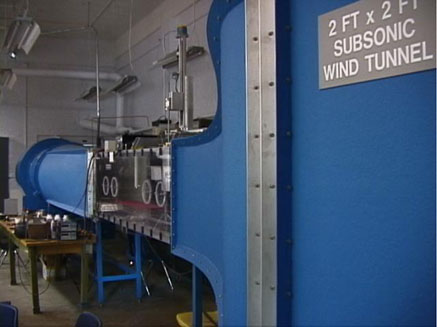
\includegraphics[width=.75\linewidth]{Figures/opencircuitwindtunnel.jpg}
  \caption{Subsonic wind tunnel in Auburn University's Aerodynamics Laboratory.}
\end{figure}

% What is an airfoil
For the aircraft presented in this thesis, a \textit{Wortmann FX 63{-}137} is used. Figure~\ref{fig:airfoil} shows the side profile. The name of the airfoil fully defines its aerodynamic shape.

% Different Wing Shapes

% Tail Shapes/ functionalities

% Flaps, what do they do, how do they work

% Wing tips

% CFD Modeling

% Strip Theory Modeling





\begin{figure}[!ht]\label{fig:airfoil}
  \centering
  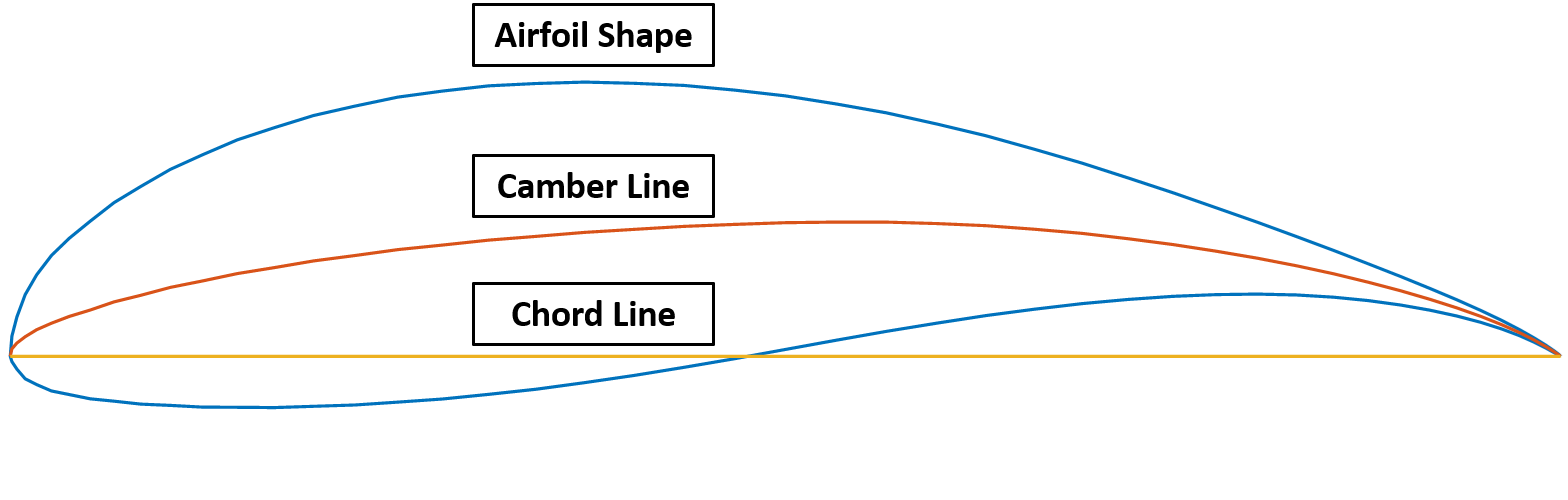
\includegraphics[width=\linewidth]{Figures/da40airfoil.png}
  \caption{Wortmann FX 63{-}137 airfoil modeled on simulated Diamond DA-40 aircraft.}
\end{figure}

\subsection{Landing Gear Model}
Although not calculated often, the modeling of the aircraft's landing gear are important and should not be overlooked. However, because of the flight paths investigated in this thesis focus solely on the aircraft during flight, a simplified dynamic model is used to describe the forces and moments acting on the landing gear during landing. It should be noted that the aerodynamic calculations of the landing gear occur in the aerodynamically modeling section, while this section focuses on the moments and forces generated from the runway opposing the weight of the aircraft.

To describe the forces and moments generated during landing, a mass-spring damper system (Figure~\ref{fig:ldgfbd}) can be used in simulate the the struts, levers, and tire depression (Figure~\ref{fig:ldg}) that absorb much of the forces, moments and vibrations that act onto the aircraft during landing.

\begin{figure}[!ht]\label{fig:ldgfbd}
  \centering
  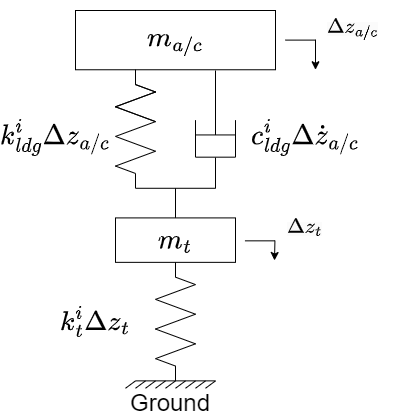
\includegraphics[width=.4\linewidth]{Figures/ldgfbd.drawio.png}
  \caption{Mass-spring damper system, representing the components of landing gear on the aircraft (adapted from~\cite{xingStrengthAnalysisDiagonal2012}).}
\end{figure}

\begin{figure}[!ht]\label{fig:ldg}
  \centering
  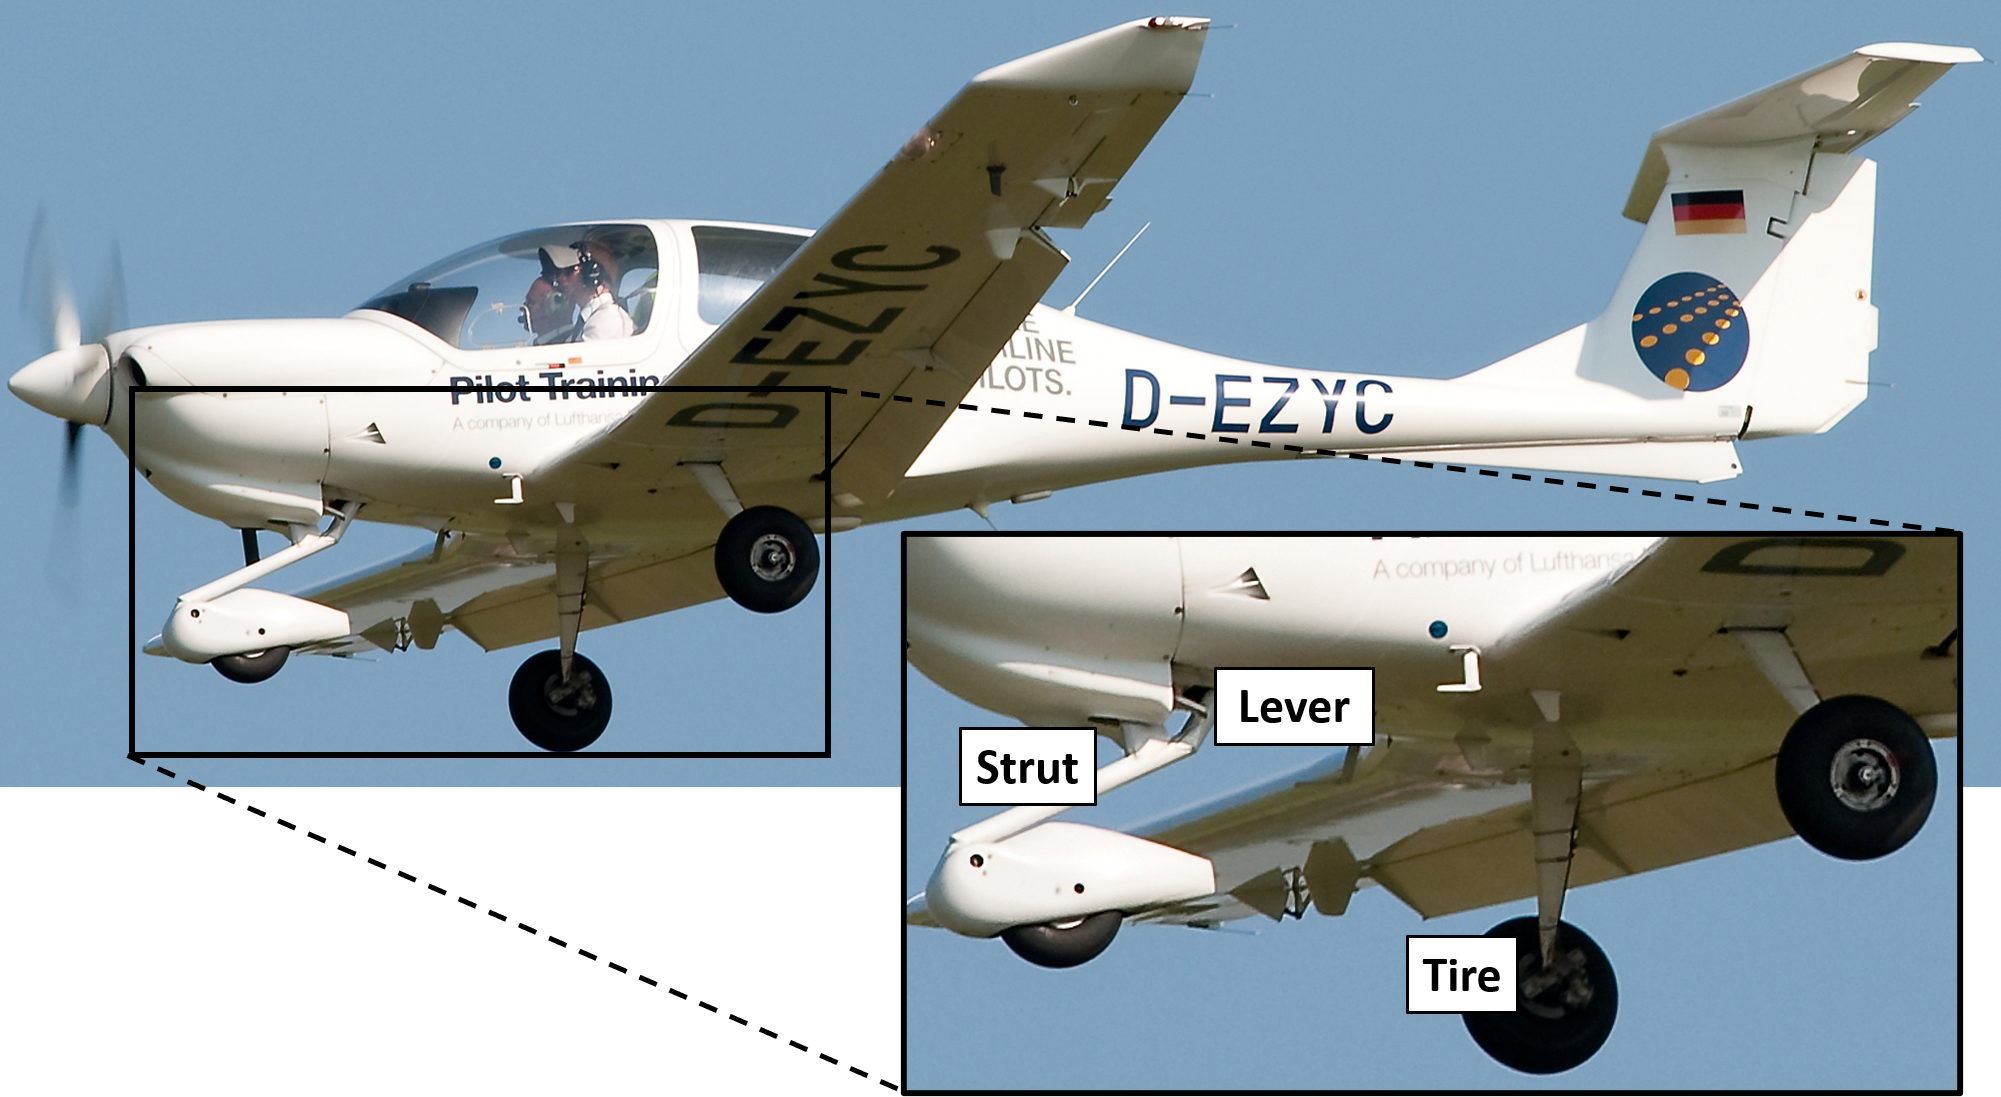
\includegraphics[width=.75\linewidth]{Figures/LandingGear.png}
  \caption{Identification of the landing gear components on the Diamond DA40.}
\end{figure}

Expanding Newton's second law, the forces on each landing gear are solved in the vertical direction (Equation~\ref{eq:ldgforces})

\begin{equation}
  \sum F^i_z = m\,a_z = k^i_t\, \Delta z_t\, + \, k^i_{ldg}\, \Delta z_{a/c}\, + c^i_{ldg}\, \Delta \dot{z}_t,
  \label{eq:ldgforces}
\end{equation}

where \(k^i_{ldg}\) and \(c^i_{ldg}\) are the spring and damper coefficients of the struts and levers respectively (see Table~\ref{tbl:ldgcoeff} for the values used in this simulated model). \(\Delta z_{a/c}\) and \(\Delta \dot{z}_t\), are the deflection and rate of deflection of the aircraft during landing.\( k^i_t \) and \(\Delta z_t\) are the tire \textit{spring} coefficient and tire depression respectively. For a general aviation aircraft, the depression of the tire upon landing is relatively small such that this term is thrown out.

\begin{table}[!ht]\label{tbl:ldgcoeff}
  \caption{List of spring and damper coefficients for nose and rear landing gear.}
  \centering
  \begin{tabular}{cccc}
    \toprule
    \textbf{i} & \textbf{Location} & \(\mathbf{k}\) \(  \left[\frac{kN}{m}\right]\) & \(\mathbf{c}\) \( \left[\frac{kN\,s}{m}\right]\) \\
    \midrule
    1          & Nose              & \(50\)                                         & \(11.3\)                                         \\
    2          & Rear Right        & \(80\)                                         & \(14.3\)                                         \\
    3          & Rear Left         & \(80\)                                         & \(14.3\)                                         \\
    \bottomrule
  \end{tabular}
\end{table}

The observed moments are solved by taking the cross product between the calculated forces of each landing gear and the moment arm (Equation~\ref{eq:ldgmoments}).

\begin{equation}
  \sum M^i = \textnormal{cross}([\,0\,;\,0\,;\,F^i_z\,],[\,x^i\,;\,y^i\,;\,z^i\,])
  \label{eq:ldgmoments}
\end{equation}

In Equation~\ref{eq:ldgmoments}, \(x^i\), \(y^i\), and \(z^i\) represent the moment arm that is derived from the center of gravity for the aircraft down to where each tire makes contact with the ground.

As a final note, it should be made clear that the forces and moments that act upon the landing gear if and only if a tire has made contact with the ground, for computational efficiency.

\subsection{Forces and Moments Calculations}
The final product of all the aforementioned systems sums to 2 things~-~the forces and moments acting on the body of the aircraft. This work demonstrates the high-fidelity modelling of engines, propellers, landing gear, and aerodynamic forces and moments the simulated flight vehicles generates while in flight. The final step of these calculations is to add them together in the body-fixed \(X\), \(Y\), and \(Z\) directions. This is demonstrated by Equation~\ref{eq:sumForce} and Equation~\ref{eq:sumMoments}.

\begin{equation}
  \sum \mathbf{F} = \mathbf{F}_{prop} + \mathbf{F}_{aero} + \mathbf{F}_{LDG}
  \label{eq:sumForce}
\end{equation}

\begin{equation}
  \sum \mathbf{M} = \mathbf{M}_{prop} + \mathbf{M}_{aero} + \mathbf{M}_{LDG}
  \label{eq:sumMoments}
\end{equation}

It should be noted that \(\mathbf{F}_{LDG}\) and \(\mathbf{M}_{LDG}\) are only calculated when the aircraft is landing.

Once the forces and moments are calculated, linear and angular velocities, along with their respective positions can be calculated.
\clearpage

\section{Guidance System}
For commercial flights, it is important for the aircraft to know where the final destination is and how to fly there in an efficient and effective manner. These questions are usually answered by the guidance system and the pilots are provided a flight plan before taking off. The guidance system provides a time series of instructions to feed into the aircraft control to mandate the speed of the aircraft, the altitude of the aircraft, and what radius to bank about with making turns along the journey to the final destination. A similar guidance system is implemented for simulated flight vehicle demonstrated in this thesis.

\subsection{Waypoint Generation}

\subsection{Calculating Controller Commands}

\clearpage
\section{Control Scheme}

\clearpage
\section{Sensor Modeling}
\subsection{Onboard sensors}

\clearpage
\chapter{GPS Simulator and Software Defined Receiver}
Since 1993, the Global Positioning System (GPS) has provided users with capable hardware to determine their global position within seconds and in recent developments, a centimeter-level position error. GPS can be explained in 3 components: the satellite vehicles in space, control and transmission of signals, and the receiver processing component.

GPS satellites have undergone multiple improvements and upgrades since the first satellites were launched in 1978. These versions of satellites are based on their \textit{block}. Currently, Block III is the most advanced satellite orbiting Earth today. Early versions (Block I) of GPS satellites were used mainly for development and did not transmit signals to the public. Lessons learned from the Block I satellites were fully integrated into the Block II GPS satellites, where GPS became fully operational in 1993. While there were many subtle differences between Block I and Block II satellites, the most important difference is that these new satellites broadcasted a signal on 2 frequencies, coined \textit{L1}, \textit{L2}, and \textit{L2c}, where \textit{L2c} is intended for civilian use. Modern day Block III satellites transmit their signal on the same frequencies that Block II satellites have, with the addition of \textit{L5}. Table provides the frequencies that signals are transmitted on.

\begin{table}[h!]\label{tbl:GPSfreq}
  \centering
  \begin{tabular}{lc}
    \toprule
    \textbf{Name} & \textbf{Frequency [Mhz]} \\
    \midrule
    \textit{L1}   & \(1575.42\)              \\
    \textit{L2}   & \(1227.60\)              \\
    \textit{L2c}  & \(1227.60\)              \\
    \textit{L5}   & \(1176.45\)              \\
    \bottomrule
  \end{tabular}
\end{table}

\clearpage
\chapter{Sensor Fusion Algorithm}
%% Background/Introduction
\clearpage
\section{Sensor Fusion Architectures}
% Types of Sensor Fusion algorithms
\clearpage
\section{Deeply Coupled GPS and FVDM Navigation Filter}
% Deeply Coupled Integration
\subsection{Update \textit{a priori}}
% Time Update
\subsection{Update \textit{a posteriori}}
% Measurement Update
\subsection{Fault Detection}
% fault Detection and Exclusions
\clearpage
\chapter{Scenario Implementation and Results}
\clearpage
\chapter{Conclusion and Future Work}
\clearpage
\appendix
\chapter*{Appendix A\addcontentsline{toc}{chapter}{Appendices}}
\begin{figure}\label{fig:atmos}
  \centering
  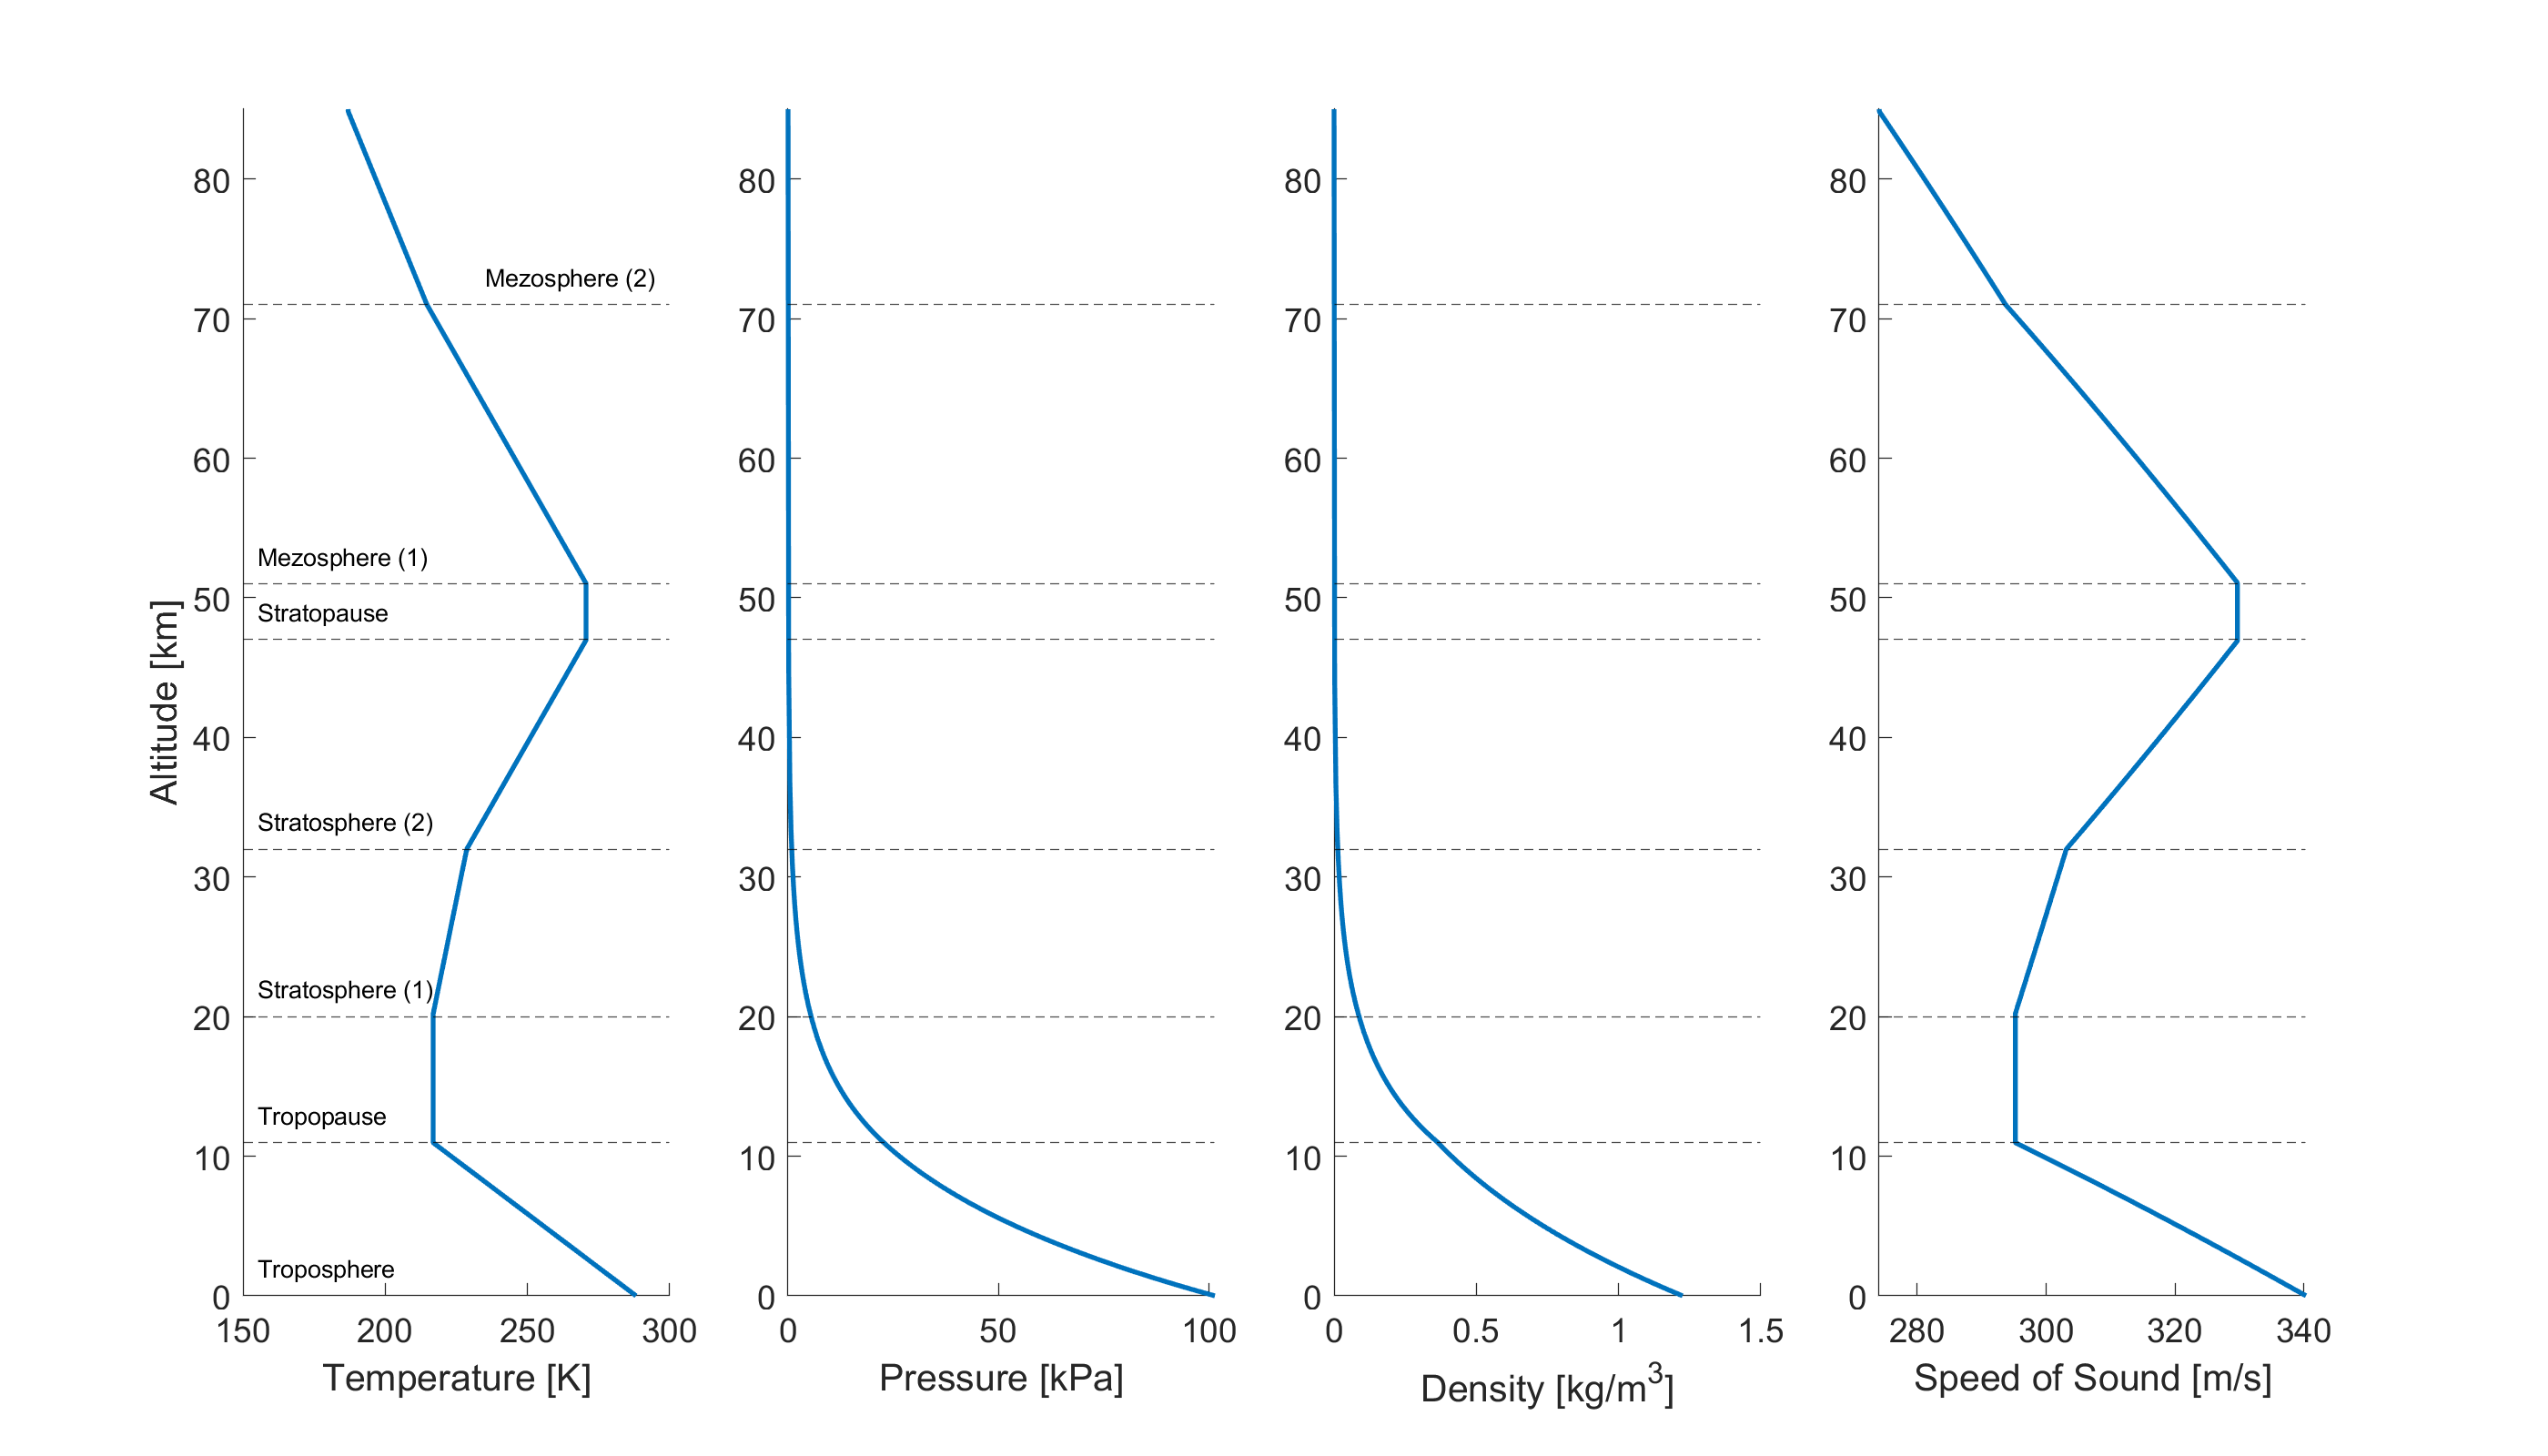
\includegraphics[width=\linewidth]{Figures/atmosphericparameters.png}
  \caption{Absolute temperature, ambient pressure, air density, and speed of sound using the ISA model.}

\end{figure}

\printbibliography{}

\end{document}

